
\chapter{Results}
% LC 25pgs
\label{Results} 

%This chapter presents the outputs that you produced, by applying the methods that you have selected, including e.g. analysis, design, prototyping, experimental work, evaluation, etc.  
  
%How you report these results will depend on the nature of the work. It may be helpful to divide them into basic data (e.g., for a project that developed a software product, requirements specification, test data, etc.) and analysis of the data (e.g. statistical analyses, evaluation analyses, etc.). Remember that you are informing the reader of what you have produced and found and emphasising the interesting parts, 
% IMPORTANT - ADD SUMMARIES
% so summarising at the end of each major section is useful.  
  
%It is usually very helpful for the readers to include graphics and diagrams, for instance to clarify software design or requirements, identify key trends and relationships in empirical data, etc. If you do so, be sure to refer to these figures in the text and use them as evidence to support what you are explaining or arguing; and be sure that your figures are well designed and clearly presented – do not just use default settings of the software you are using in producing them.  
  
%It is essential that you identify clearly what you accomplished or produced yourself, as opposed to what existed before you started your individual project or was provided by others. For instance, some projects build new software on top of an existing code base, add new data to an existing body of data, or are executed by a student as a member of a team. It is essential to indicate what parts of the activities and results which you report are your own work. If this is left unclear, the markers are instructed not to give credit for work that they cannot attribute to you. Ambiguity would attract penalties for poor academic practice, with delays caused by any investigation (deception would be treated as academic misconduct, of course, which may lead to expulsion).

% Feedback from Artur Garcez with respect to Results
% The most important thing now is to describe clearly (with the right level of detail - not too much, not too little) the (...) evaluation of results (there's a more objective evaluation here of accuracy/speed but also a subjective evaluation that you can discuss in more detail: when a situation changes from "no rain" to "rain" and how that affects the pre-trained network). With those results you will have the material needed for the important discussion chapter which should include your own critical evaluation of results and also point to future work.

%%%%%%%%%%%%%%%%%%%%%%%%%%%%%%%%%%%%%%%%%%%%%%%%%%%%%%%%%%%%%%%%%%%%%%%%%%%%%
% OUTPUTS
%%%%%%%%%%%%%%%%%%%%%%%%%%%%%%%%%%%%%%%%%%%%%%%%%%%%%%%%%%%%%%%%%%%%%%%%%%%%%

\section{Outputs}
Since this dissertation's topic first took shape (\ref{corr_with_super}) a number of outputs were generated, not all recorded or saved. With respect to outputs that were recorded and saved, this project generated five classes of outputs: 1. models, 2. videos, 3. tcpflow logs, 4. synthetic datasets and 5. code. A number of "Runs" were recorded in \ref{res:training_and_testing_log}. A run may or may not generate a model, may or may not generate a video and may or may not generate a tcpflow log. A model may be run several times, as were the best nvidia1 (\ref{app_res:49}) and nvidia2 (\ref{app_res:62}) models, tested with different levels of rain and light intensity multipliers.
A compilation of saved models, videos and tcpflow logs, shown in \ref{app_res:outputs} lists 73 models, 61 published (YouTube) videos and 30 tcpflow logs at the time of compilation. Public download links are available in \ref{res:download-links}.

%%%%%%%%%%%%%%%%%%%%%%%%%%%%%%%%%%%%%%
% DATASETS
%%%%%%%%%%%%%%%%%%%%%%%%%%%%%%%%%%%%%%

\section{Datasets}

The following training unity datasets were generated:
\begin{verbatim}
$ . count.sh 
871403 files in directory .
25562 files in directory ./roboRacingLeague
25795 files in directory ./log_sample
82245 files in directory ./warehouse
44496 files in directory ./quarantine
90842 files in directory ./smallLoop
516997 files in directory ./genRoad
16570 files in directory ./genTrack
68886 files in directory ./smallLoopingCourse
\end{verbatim}
where approximately half are the labels (.json files) so the total number of images generated is 435701 while the most used for training and testing were genTrack and genRoad for an approximate total of 266783 images used to train the best performing models. In addition to Generated Track and Generated Road, the RoboRacingLeague and Warehouse tracks were also attempted and could have potentially worked. In the end to keep the problem constrained, two tracks were used.
%Directory           Number of files Comment
%smallLoopingCourse/ 34443           from small_looping_course
%warehouse/          41126           From Warehouse course
%smallLoop/          45422           From small_looping_course
%roboRacingLeague/   12778           From "Robot Racing League" course
%log_sample          25791           From small_looping_course
%genRoad             280727          From "Generated Road" course
From the real life datasets considered, Audi, FordAV, Kitti and Udacity. All were inspected and notes made in \ref{appA:datasets} and the dissertation latex directory work-diary.txt. Correspondences were held with authors (\ref{corr_with_authors}) with respect to extracting steering angles from datasets, and ROS (Robot Operating System) was used to extract data from public dataset files provided in the rosbag format (\ref{appA:FordAvDataset}). 
%the overall conclusion being there were too many disparate formats to deal with, though it was interesting to use ROS (robot operating system) to extract sensor data from rosbag files. Another problem was no rainy images were implied to exist in any of these public datasets.

%%%%%%%%%%%%%%%%%%%%%%%%%%%%%%%%%%%%%%%%%%%%%%%%%%%%%%%%%%%%%%%%%%%%%%%%%%%%%
% Mechanical Turk
%%%%%%%%%%%%%%%%%%%%%%%%%%%%%%%%%%%%%%%%%%%%%%%%%%%%%%%%%%%%%%%%%%%%%%%%%%%%%

\section{Locating rainy sections with Mechanical Turk}
\label{res:mech-turk}
To investigate the effect of rain in self-driving CNNs in a real world dataset, an attempt was made to locate such images in available autonomous vehicle public datasets.
The data that looked most promising was Ford V2 Log 1 and V3 Log 1 from the FordAV dataset (\cite{agarwal2020ford}), both described as "freeway, overpass, bridge, cloudy". The goal was the set to label a sample of the cloudy images with Amazon Mechanical Turk and 50 images were uniformly drawn from each log, plus 5 images with rain added with the Automold library using the RainyImagesDissertationPlot.ipynb script. The expectation being the 5 extra images be labelled as "Rain". The 105 images were then added to a SageMaker Ground Truth job. The platform works as a wrapper around Mechanical Turk as it facilitates the creation of user interfaces (Figure \ref{fig:MechTurkCreateJob})
% rainy files created with automold/RainyImagesDissertationPlot.ipynb
\begin{figure}[h!]
\centering
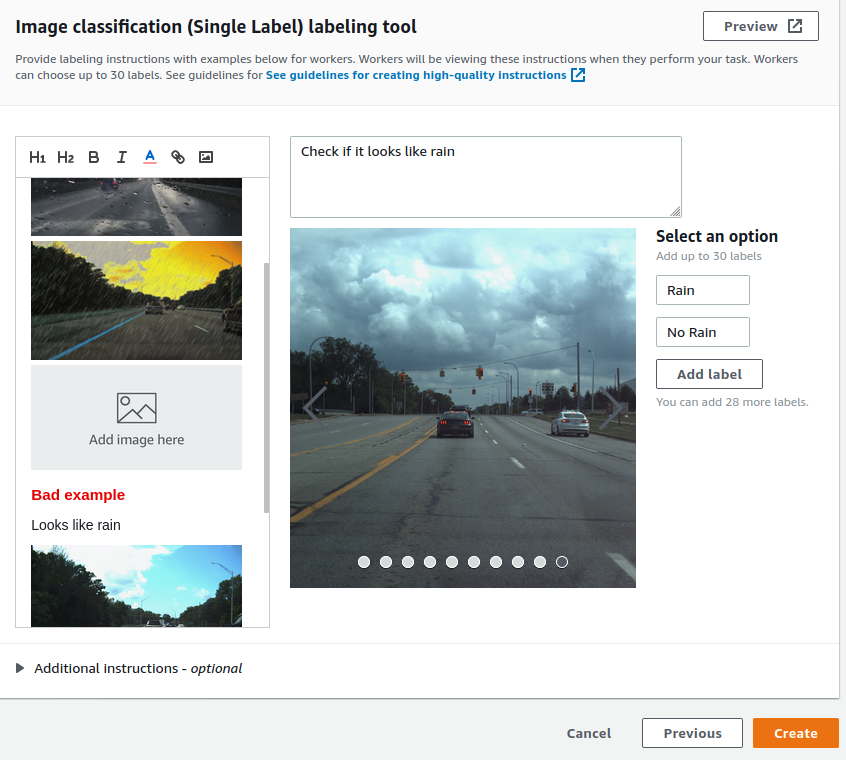
\includegraphics[width=10cm]{Figures/MechTurkCreateJob.png}
\caption{The SageMaker Ground Truth user interface template with two labels ("Rain", "No Rain"), the image to be labeled and examples of correct and incorrect classifications. On the top left are images supplied as "Good example" of rain. The lower of the two being an image modified with the Automold library to add rain. After the job was submitter, the image was labelled by a Mechanical Turk worker as "No Rain".}
\label{fig:MechTurkCreateJob}
\end{figure}
Labelling tasks are classified as low, medium and high complexity. The prices range from \$0.012 for a low complexity task, with a 5 second estimate to complete, to \$1.20 for a high complexity task with a 3.5 minute estimate to complete.
The task can be configured with an output for time taken by a worker on a single task, the lowest time interval being one minute.
There is also an option to assign more than one worker per dataset object, on account that it can help increase the accuracy of the data labels.
The task was created with the most basic options of one worker, a \$0.012 price per task, a one minute timeout and remained live for 12 hours. 
The images were labelled by one Mechanical Turk worker and results made available in a json encoded file (dataset/mechanical-turk/2020-11-21\_22 45 37.json). In case more than one worker is assigned to a same task, a confidence score is also provided in the results. Results showed no images had been labeled as "Rain". The assumption then being there are no sections containing rain in the dataset. The Automold library added rain images were also labeled as "No Rain" by the worker. Figure \ref{fig:MechTurkLabeledImages} shows one page of the SageMaker Ground Truth completed job, detailing 4 labelled images on the Labeling Job Summary page. A side-effect of the labelling job being Automold rain where not seen by a human as such. The implication is further discussed in \ref{Discussion}.
\begin{figure}[h!]
\centering
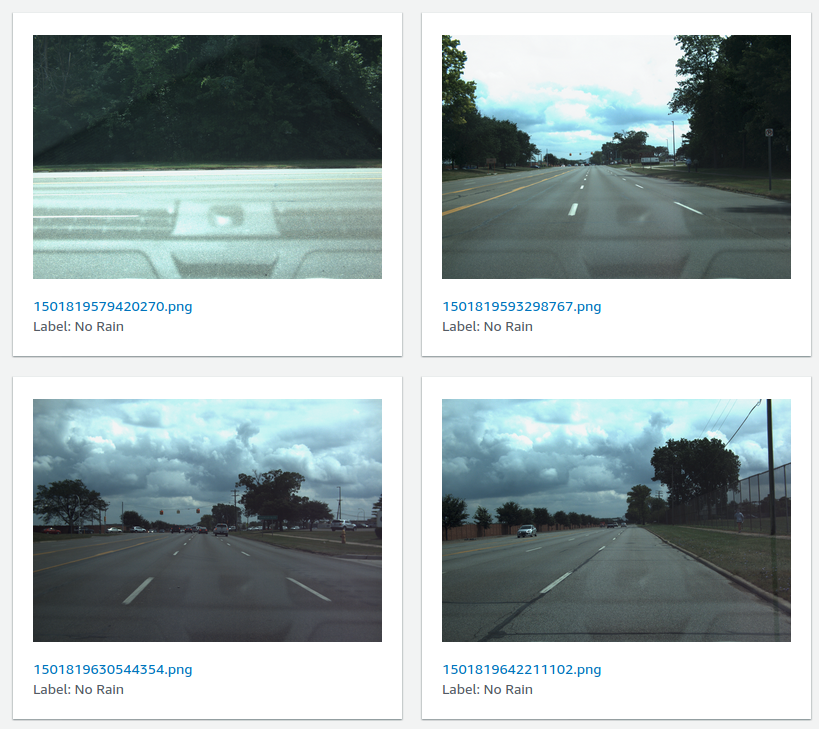
\includegraphics[width=10cm]{Figures/MechTurkLabeledImages.png}
\caption{The SageMaker Ground Truth labeled images detail on Labeling Job Summary page}
\label{fig:MechTurkLabeledImages}
\end{figure}


%%%%%%%%%%%%%%%%%%%%%%%%%%%%%%%%%%%%%%%%%%%%%%%%%%%%%%%%%%%%%%%%%%%%%%%%%%%%%
% PRODUCING A SELF-DRIVING MODEL
%%%%%%%%%%%%%%%%%%%%%%%%%%%%%%%%%%%%%%%%%%%%%%%%%%%%%%%%%%%%%%%%%%%%%%%%%%%%%
% The story we are telling:
% 1. how we used SDSandbox to produce data and what the steering data looked like
% 2. How we trained the models
% 2. How we added rain to the data
% 3. How we drove in the rain and what the steering data looked like
\section{Generating Synthetic Datasets} % with SDSandbox} this should be obvious by now

%%%%%%%%%%%%%%%%%%%%%%%%%%%%%%%%%%%%%%%%%%%%%%%%%%%%%%%%%%%%%%%%%%%%%%%%%%%%%
% SYNTHETIC DATASETS
%%%%%%%%%%%%%%%%%%%%%%%%%%%%%%%%%%%%%%%%%%%%%%%%%%%%%%%%%%%%%%%%%%%%%%%%%%%%%

\subsection{Generated Track}
Figure \ref{fig:GeneratedTrackPlusHist} shows a normalized histogram of 45410 steering angles obtained in 10 recorded sessions (data directory dataset/unity/smallLoop) for the small\_ looping\_ circuit track seen on the right. The circuit is the same as the Generated Track circuit, while the landscape in the latter excludes trees, bushes and tall grass. The simulator records at a, computational resources allowing, maximum rate of 60 fps (frames per second). The observed average on the track was approximately 24 fps, representing in this case 31m32s of recorded data in approximately 19 laps. The 24 fps average was obtained by recording ("Auto Drive w Rec" option) for one lap, taking approximately 1m41s seconds and generating 2455 frames. The simulator registered fps rates higher than average on straight sections and lower than average on curved sections. This is assumed to be due to computational overheads imposed on the physics engine in the curved sections, resulting in less frames being processed and recorded. The maximum steering angle is set in the simulator with respect to a car. In this case it is plus or minus 25 degrees. The normalized value, in the range of -1 to 1 is recorded. Values displayed in the histogram are multiplied by the maximum steering angle, referred to in this study as the \textit{normalization constant}. The data shows a high bias towards positive steering angles because the simulated vehicle drives clockwise around the track. From the starting line on the top left, there are two right turns, followed by a left turn, followed by two right turns.
\begin{figure}[ht]
 \centering 
 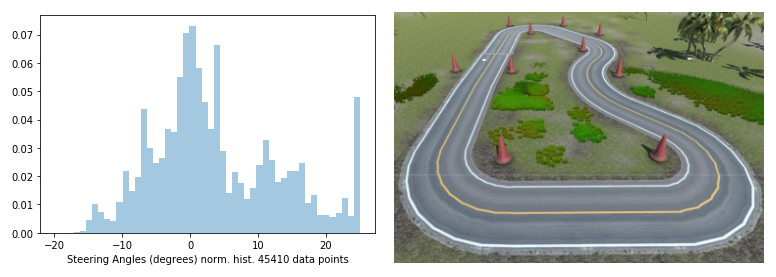
\includegraphics[width=\textwidth]{Figures/GeneratedTrackPlusHistogram.png}
 \caption{Normalized histogram of Unity 3D SDSandbox steering angles for 45410 image frames. The corresponding track (small\_looping\_couse) is shown on the right}
 \label{fig:GeneratedTrackPlusHist}
\end{figure}

Figure \ref{fig:genTrackOneLap_logs_Wed_Nov_25_23_39_22_2020_ground_truth_steering_angles} shows the \textit{ground truth} (not predicted) steering angles obtained in "Auto Drive w Rec" mode, for one lap driven around the Generated Track, saved to log directory dataset / Unity / genTrack / logs\_ Wed\_ Nov\_ 25\_ 23\_ 39\_ 22\_ 2020 made available for download in \ref{res:download-links}. The y axis is inverted such that plot follows steering adjustments, if observer tilts head to the right. The four troughs  represent the four right turns. The hump between frames 500 and 700 represents the only (gentle) left turn in the circuit, where the steering angle is keep negative while the vehicle negotiates the bend.

% NB Table gos data and figures generated with code commit hash cc095fc
% Figure generated with GetSteeringAnglesFromtcpflow.ipynb
\begin{figure}[ht]
 \centering 
 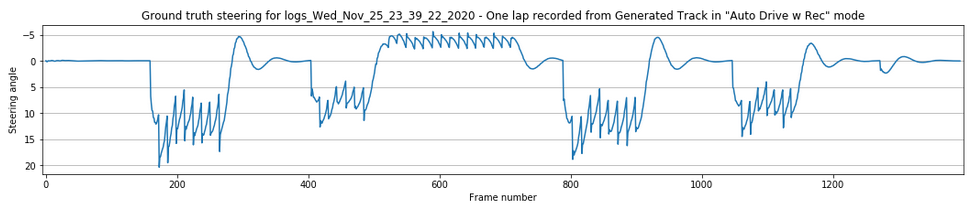
\includegraphics[width=\textwidth]{Figures/genTrackOneLap_logs_Wed_Nov_25_23_39_22_2020_ground_truth_steering_angles.png}
 \caption{Ground truth steering values for logs\_ Wed\_ Nov\_ 25\_ 23\_ 39\_ 22\_ 2020 recorded log.}
 \label{fig:genTrackOneLap_logs_Wed_Nov_25_23_39_22_2020_ground_truth_steering_angles} 
\end{figure}

\subsection{Generated Road}
Another simulated circuit used was the \textit{Generated Road}, which creates a random path on every run. This can be seen in figure \ref{fig:GeneratedRoadPlusHist}. The total number of frames collected for 15 \textit{Auto Drive w Rec} sessions (saved in dataset/unity/genRoad) was 280727, approximately 3h14m37s. The outliers, mainly to left of histogram, are due to the simulated vehicle being left unattended, reaching the end of the road and continuing into a section with no road markings, becoming stuck in a hard-left turn, until the simulation was switched off and recording halted. The mean and standard deviation, for angles in the range -20 to + 20 (excludes outliers), are -0.18 and 5.37 degrees respectively. The number of outliers omitted from the plot (not excluded from data at this stage) was 2204 (0.79\%). It can be seen that when more data points are collected, the histogram becomes "smoother", if compared to equivalent plot in Figure  \ref{fig:GeneratedTrackPlusHist}.
Both boths are clearly centered around zero degrees, meaning the vehicle is driving straight more often than not. The Generated Road has a normally distributed steering angle distribution because of the same number of left and right turns in the circuit, which infers the data distribution is track-dependant.

\begin{figure}[ht]
 \centering 
 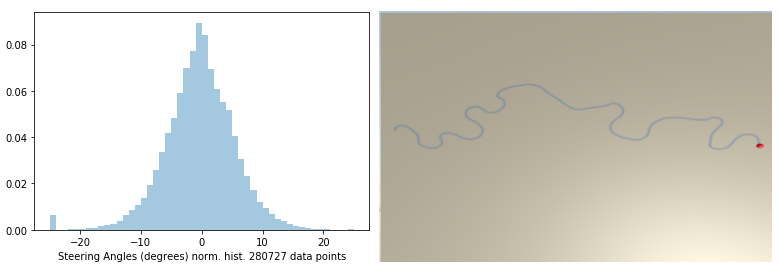
\includegraphics[width=\textwidth]{Figures/GeneratedRoadPlusHistogram.png}
 \caption{Normalized histogram of Unity 3D SDSandbox generated road, steering angles for 280727 image frames. A sample randomly generated road is shown on the right. Outliers in negative range are due to oversteering when vehicle reached the end of the road and simulator was left recording.}
 \label{fig:GeneratedRoadPlusHist}
\end{figure}

\section{Training self-driving models}
Model training was performed using a modified version of the SDSandbox/src/train.py script. A successful training run produces four files: a plain text .log file containing the script running time duration and last recorded values of accuracy and loss for training and validation (the training "history"), a .history file in the pickle format containing all history values, a model .h5 file in the pickle format containing the model structure and weights, and a .png image file containing a history plot for the training run.
Figure \ref{fig:devcloud_nvidia2__camber_baseline_local_sanity_accuracy} shows three training history plots: 20201124032017\_ nvidia2.h5 trained for 23 epochs on the Intel DevCloud, 20201121090912\_ nvidia\_ baseline.h5 trained for 2 epochs on Camber and 20201120184912\_ sanity.h5 trained for 82 epochs on the local workstation. The left y axis represents loss and the right y axis represents accuracy values. The x axis represents training epochs (one run through the entire dataset). The title for each plot contains the last recorded training history values and the model name.
\begin{figure}[ht]
 \centering 
 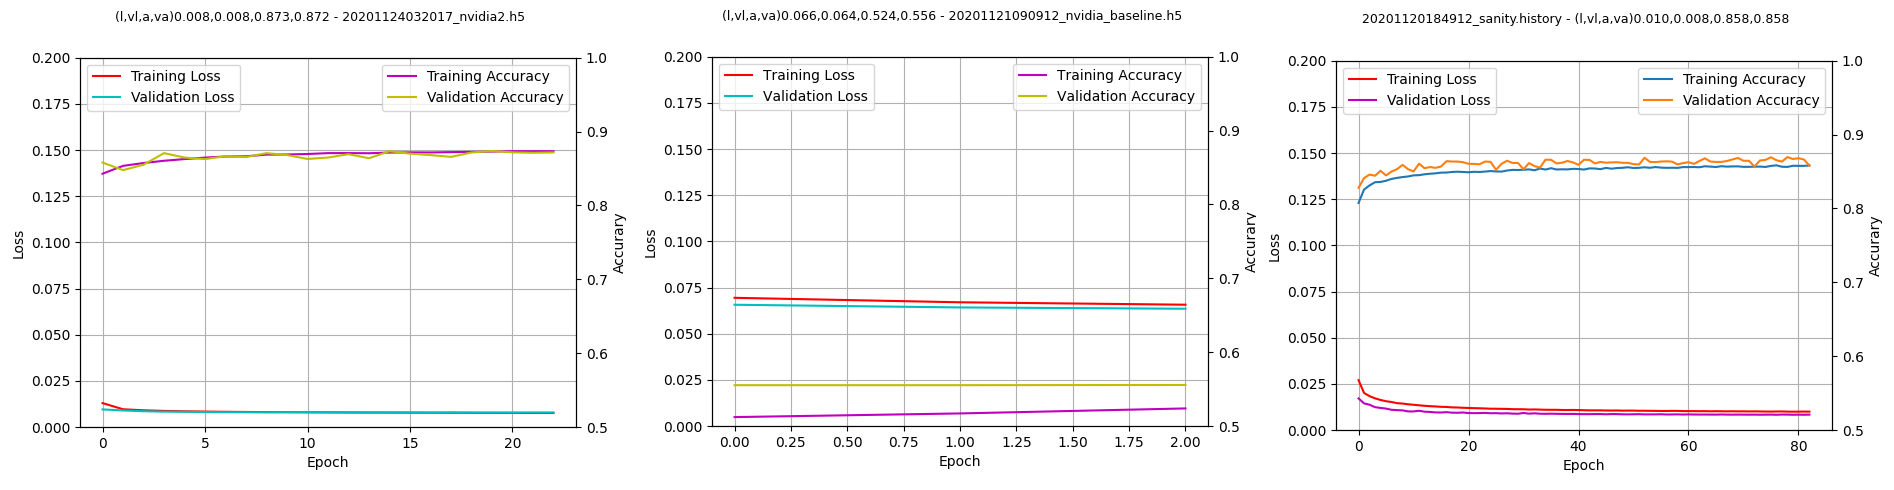
\includegraphics[width=\textwidth]{Figures/devcloud_nvidia2__camber_baseline_local_sanity_accuracy.png}
 \caption{Training and validation accuracy and loss value plots for, left to right, models 20201124032017\_ nvidia2.h5, 20201121090912\_ nvidia\_ baseline.h5 and 20201120184912\_ sanity.h5}
 \label{fig:devcloud_nvidia2__camber_baseline_local_sanity_accuracy}
\end{figure}

Listing \ref{training_logs} shows the corresponding log files for each run, training run documented in \ref{app_res:62} (devcloud), \ref{app_res:98} (camber) and \ref{app_res:37} (local) respectively.

\label{training_logs}
\begin{verbatim}
Model name: ../trained_models/nvidia2/20201124032017_nvidia2.h5
Total training time: 4:06:55
Training loss: 0.008
Validation loss: 0.008
Training accuracy: 0.873
Validation accuracy: 0.872

Model name: ../trained_models//nvidia_baseline/20201121090912_nvidia_baseline.h5
Total training time: 0:05:25
Training loss: 0.066
Validation loss: 0.064
Training accuracy: 0.524
Validation accuracy: 0.556

Model name: ../trained_models/sanity/20201120184912_sanity.h5
Total training time: 16:08:01
Training loss: 0.010
Validation loss: 0.008
Training accuracy: 0.858
Validation accuracy: 0.858 
\end{verbatim}

Training and validation data was split at 80\%/20\% ratio. Early stopping was used with patience typically set to 6 epochs for validation loss (stop if no decrease over 5 epochs). Images were presented to network in batches of 64. The Adam optimizer was used with a learning rate of 0.0001 and mean squared error loss function. Trainnig and testing runs are documented in appendix \ref{AppendixD}.

%%%%%%%%%%%%%%%%%%%%%%%%%%%%%%%%%%%%%%%%%%%%%%%%%%%%%%%%
% Testing self-driving models without rain
%%%%%%%%%%%%%%%%%%%%%%%%%%%%%%%%%%%%%%%%%%%%%%%%%%%%%%%%
\section{Testing self-driving models without rain}
To create a proof-of-concept, the initial model architecture used was TawnNet. In the documentation, the author states that with the SDSandbox framework, self-driving was achieved with a few hours of recorded laps and up to one day (24 hours) training time on GPU, with the code supplied "as is". This experiment was replicated (20.07.2020 on CPU) while the outcome was not as the car, after initially staying on the Generated Road, drove off the track. The experiment recorded in video  \url{https://youtu.be/453mTlL2gvs}.    

The first working model (able to successfully self-drive around the Generated Track) was the 20201107210627\_ nvidia1.h5, with the nvidia1 (TawnNet) model on 07.11.2020. A video was generated using the recording screen utility Kazam (\cite{Kazam2020}), recording at 15fps (frames per second), and published at  \url{https://youtu.be/9z0mMtOnUUc}. Figure \ref{fig:SimTCPPred}
shows 3 stills from the video containing from left to right, the game engine, the tcpflow TCP debug output and the prediction engine running. tcpflow was added to the process in this project as a debugging tool, and does not exist in the original SDSandbox.

\begin{figure}[h!]
\centering
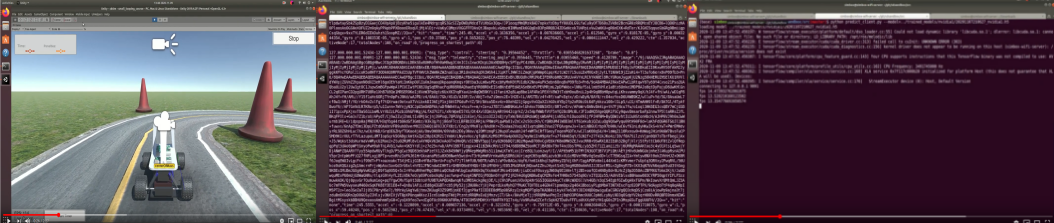
\includegraphics[width=\textwidth]{Figures/SimTCPPred.png}
\caption{Stills of video \url{https://youtu.be/9z0mMtOnUUc} showing left to right: SDSandbox simulated car going around the Generated Track course, TCP Debug (tcpflow) and prediction engine (predict\_ client.py) running}
\label{fig:SimTCPPred}
\end{figure}

A record of what code generated the successfull model was not made at the time. Forensics in \ref{app_res:36} using git logs and further tests conducted in \ref{app_res:37}, \ref{app_res:38}, \ref{app_res:39} ("sanity" models) determined it was achieved by porting the data augmentation and pre-processing described in \ref{met:data-aug-pre-proc} to the SDSandbox training and prediction scripts. The augmentation is applied during training, with a probability of 0.6, pre-processing is applied to all images. Pre-processing is applied to all images received from simulator during inference time.

Once the sanity model could successfully drive around the Generated Track, tcpflow logs were captured and used to generate the video shown in Figure \ref{fig:20201120171015_sanity_sim_network}. A script was written for this end (MakeVideo.py) and the command line call can be seen in several runs e.g. \ref{app_res:41}. The video in this case is obtained by processing all still images logged by tcpflow, as when they were sent from the simulator to the prediction engine during inference time. In MakeVideo.py, the adapted \cite{Naoki2016} augmentation library is used to pre-process the original image such that it will be the same as the image presented to the network. The predicted angle is obtained from tcpflow. Labels added to the images, then both images (original and processed) are concatenated horizontally and added to a video one frame at a time using the opencv-python module. The ratio for each individual frame in the composition is set to 800x600 pixels.
\begin{figure}[ht]
 \centering 
 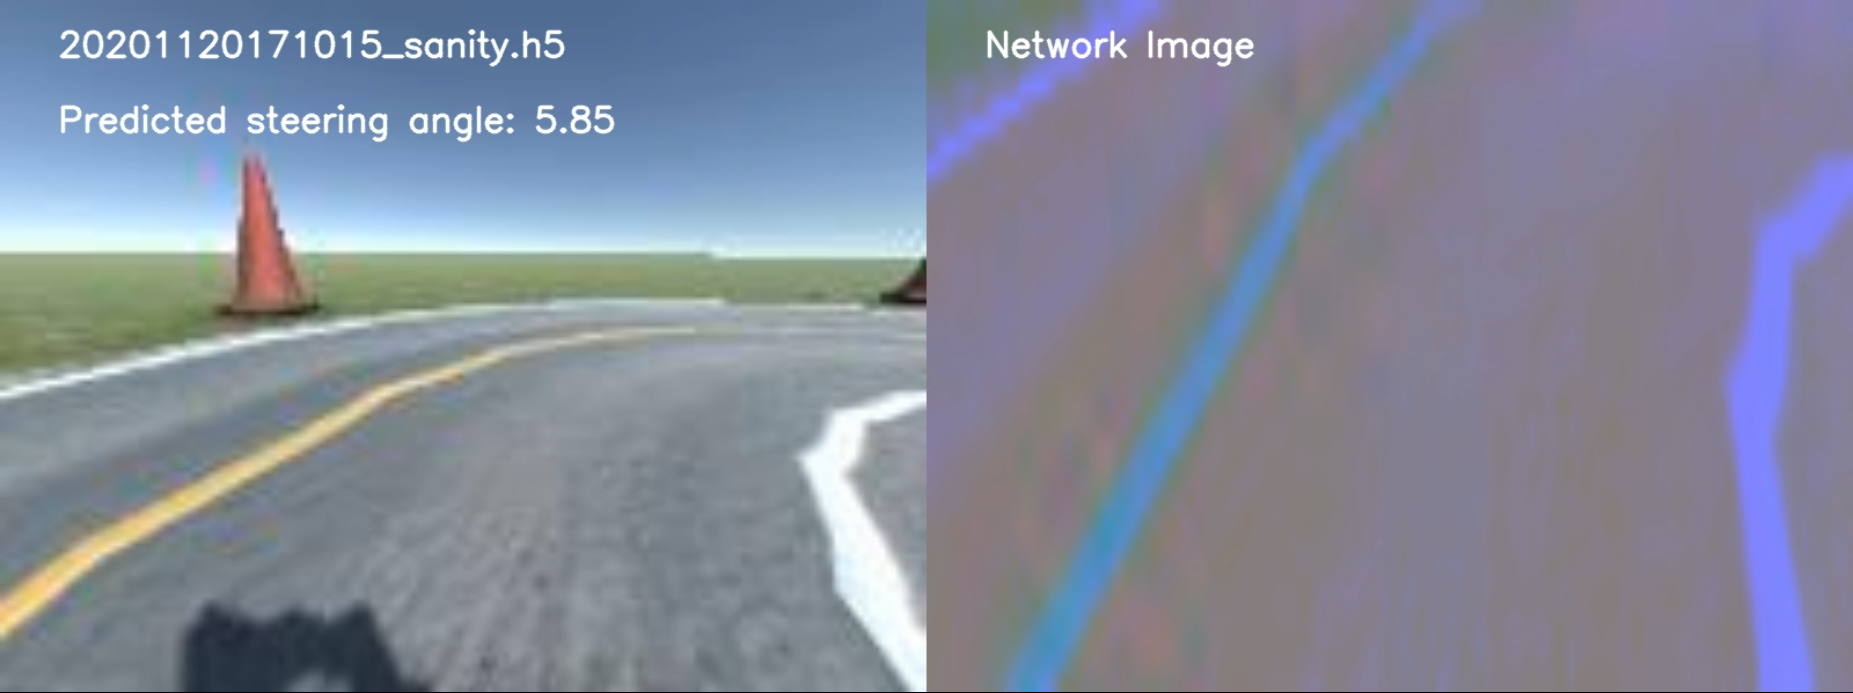
\includegraphics[width=\textwidth]{Figures/20201120171015_sanity_sim_network.png}
 \caption{Video still from run 41 video  \url{https://youtu.be/LEmZJJzJkEE} showing simulator image as sent over TCP network on the left with added CNN (20201123162643\_ sanity.h5 model) steering angle prediction and processed image (as presented to CNN) on the right}
 \label{fig:20201120171015_sanity_sim_network} 
\end{figure}

Figure \ref{fig:sa_GeneratedTrack_20201120171015_sanity} shows the plot for \textbf{predicted} steering angles around Generated Track for run 41, whereas in Figure \ref{fig:genTrackOneLap_logs_Wed_Nov_25_23_39_22_2020_ground_truth_steering_angles} shows \textbf{ground truth} steering angles are plotted. The predictions start at around 5 degrees steering slowly edging close to zero degrees. This can be observed on the video as the car moves closer to the left edge of the lane (positive steering), then continues straight.
The plot for predicted angles seems smoother than for ground truth angles. This may be due to the PID settings where the response to going off the desired path is more abrupt, and "jerkier", in trying to correct itself.

\begin{figure}[ht]
 \centering 
 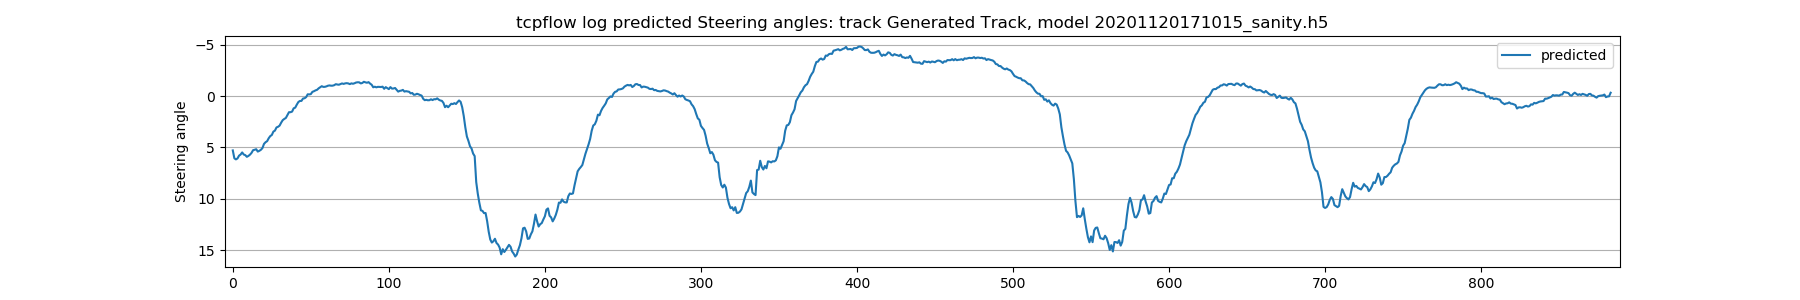
\includegraphics[width=\textwidth]{Figures/sa_GeneratedTrack_20201120171015_sanity.h5.png}
 \caption{Steering angle plot generated from tcpflow log obtained in run 41 (\ref{app_res:41})}
 \label{fig:sa_GeneratedTrack_20201120171015_sanity} 
\end{figure}

At this stage, the nvidia1 model was proven to self-drive. The nvidia2 and nvidia\_ baseline models required more work. The first step was to "clean" the genRoad dataset. % Fixing the data
Figure \ref{fig:SkewCleanup} shows from left to right, an overlay of all plots of normalized histogram plots for steering values contained in unity/genRoad directory, the folder containing most outliers (logs\_Thu\_Jul\_ \_9\_16\_00\_15\_2020) and the resulting plot once the outliers' folder was removed from unity/genRoad. 
\begin{figure}[h!]
\centering
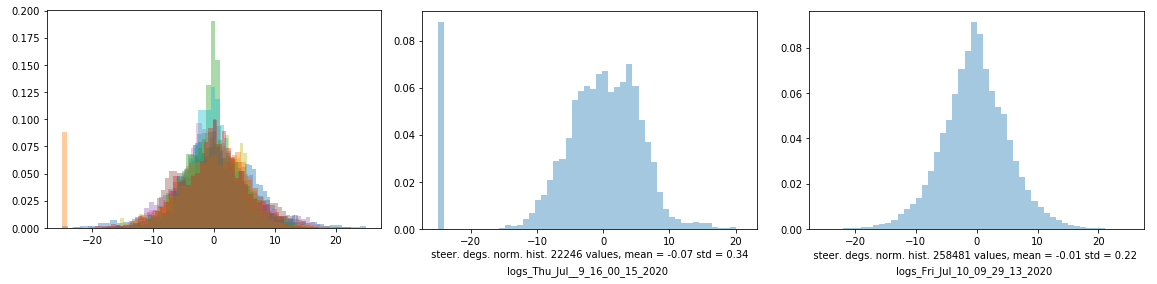
\includegraphics[width=\textwidth]{Figures/SkewCleanup.png}
\caption{Left to right, normalized histograms of all genRoad folders, outlier's folder and all data with outliers removed.}
\label{fig:SkewCleanup}
\end{figure}
The presence of outliers is believed to have caused issues with the nvidia\_ baseline model from runs \ref{app_res:15} to \ref{app_res:31}. The next issue was found to be the ratio used to crop images presented to both "problematic" networks. Run 55 (\ref{app_res:55}) provides analisys. Figure \ref{fig:nvidia1x1_nvidia2x3_crops_results} shows on the left, the crop (pre-processed image) presented to nvidia1 and sanity models. The actual crop values were determined by the imported augmentation library, which had crop values set to "frame" the "part of interest" in images (320x160) generated by the Udacity sim. The crop turned out to work for the nvidia1 and sanity models with images (160x120) generated by the SDSandbox sim, which is a "fluke": by removing 60 pixels from the top and 25 pixels from the bottom of SDSandbox images, the result was an image that seems to best frame the road. The issue was corrected by using the third crop, from left to right and a working nvidia2 model was generated in run 62 (\ref{app_res:62}). Crop values are set in script conf.py, adapted for this project.

%%%%%%%%%%%%%%%%%%%%%%%%%%%%%%%%%%%%%%%%%%%%%%%%%%
% Generated Road top crops
%%%%%%%%%%%%%%%%%%%%%%%%%%%%%%%%%%%%%%%%%%%%%%%%%%

\begin{figure}[h!]
 \centering 
 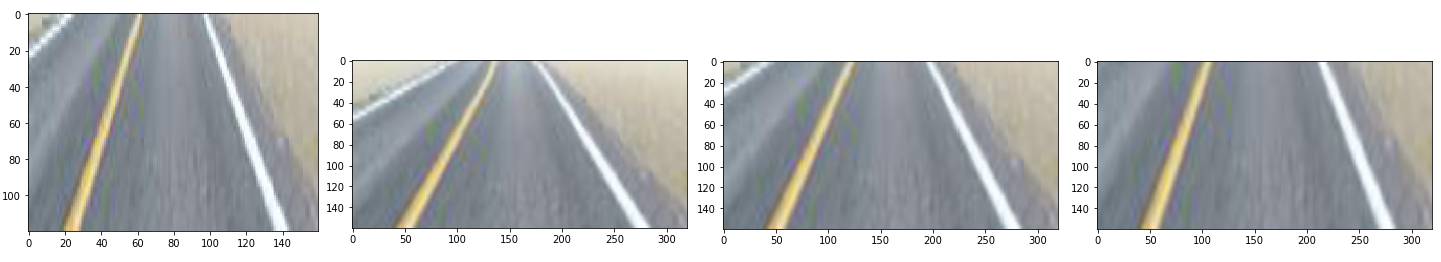
\includegraphics[width=\textwidth]{Figures/nvidia1x1_nvidia2x3_crops.png}
 \caption{Left to right, nvidia1 network crop, nvidia2 network crops at top crop set to 70, 81 and 91 pixels left to right. The 81 pixel top crop was used for the nvidia2 network}
 \label{fig:nvidia1x1_nvidia2x3_crops_results} % duplicate image
\end{figure}

Figure \ref{fig:run-93-94-generated-road-res} shows a randomly Generated Road used for runs 93, 94 and 95, where the first few hundred frames go to near the top left of the circuit (long right 180 degree turn) shown in detail on the right hand image. The predicted steering angles shown in Figure  \ref{fig:20201207192948_nvidia2_dry_genRoad} for the well performing nvidia2 20201207192948\_ nvidia2.h5 model, show the majority of values in the positive range, as the simulated vehicle follows the road and takes a right turn to do so.

%%%%%%%%%%%%%%%%%%%%%%%%%%%%%%%%%%%%%%%%%%%%%%%%%%
% Generated Road, sim on left and detail on right
%%%%%%%%%%%%%%%%%%%%%%%%%%%%%%%%%%%%%%%%%%%%%%%%%%

\begin{figure}[h!]
 \centering 
 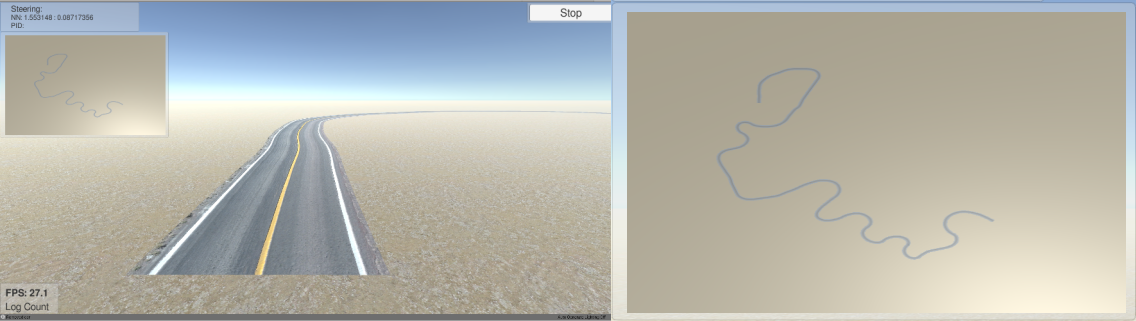
\includegraphics[width=\textwidth]{Figures/run-93-94-generated-road.png}
 \caption{The randomly generated Generated Road circuit used in runs 93 and 94. Left image is a view of the simulator as presented on computer desktop, the right image is the augmented detail showing the Generated Road circuit, the same inset on left image.}
 \label{fig:run-93-94-generated-road-res} 
\end{figure}




%%%%%%%%%%%%%%%%%%%%%%%%%%%%%%%%%%%%%%%%%%%%%%%%%%%
% ADDING RAIN
%%%%%%%%%%%%%%%%%%%%%%%%%%%%%%%%%%%%%%%%%%%%%%%%%%%

\section{Adding rain}
\label{res:adding-rain-section}
Using the Automould library, scrip predict\_ client.py was modified for rain to be added in real time for predictions. Two schemes were considered. The first where rain is added directly to the network image, as show in Figure \ref{fig:tcpflow_Run43}. Although the procedure introduces noise to images, it is somewhat unrealistic, as rain is expected to be present on the acquired image.
\begin{figure}[ht]
 \centering 
 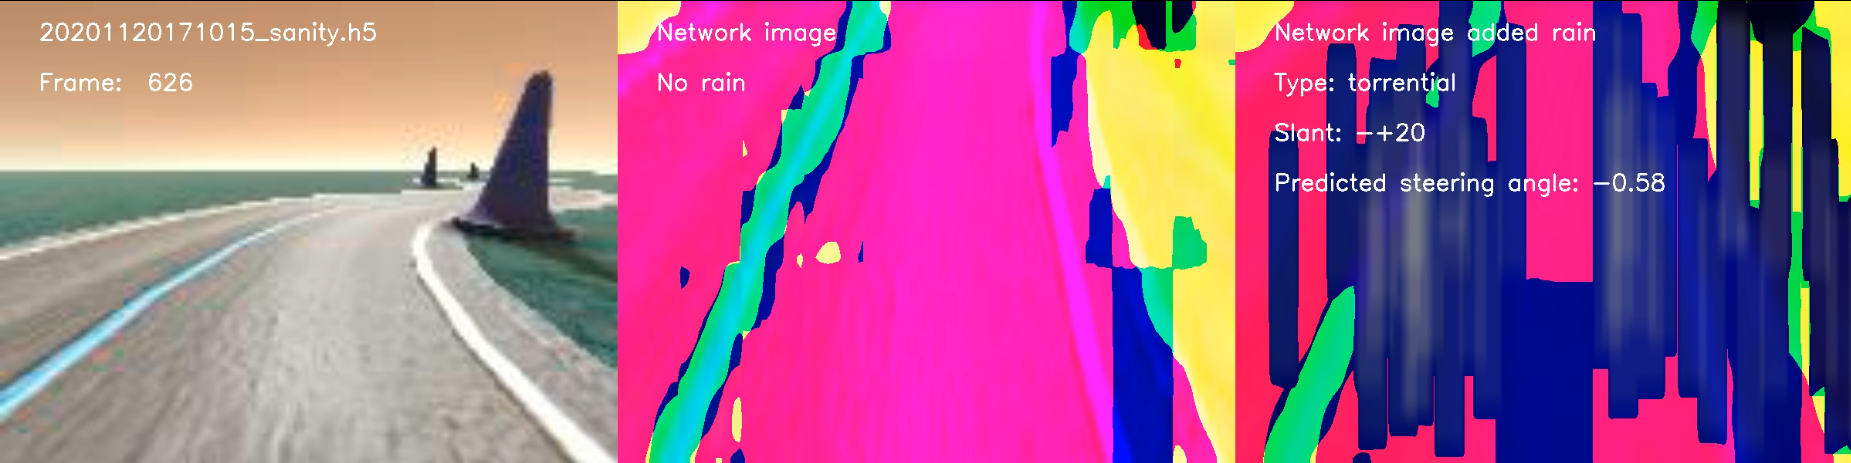
\includegraphics[width=\textwidth]{Figures/tcpflow_Run43.png}
 \caption{Video still showing left to right, the acquired image supplied by the simulator, a processed network image with no rain and the same image with torrential rain added. This last being the image presented to the network. A video was recorded in run \ref{app_res:43}, \url{https://youtu.be/57jwwcjbfdE}, showing the model driving off the track.}
 \label{fig:tcpflow_Run43} 
\end{figure}
The second scheme, adopted for this project, was adding rain to the acquired image. This is shown in Figures  \ref{fig:youtube20201207091932nvidia1lightrainmult_4_h5},
\ref{fig:youtube20201207091932nvidia1heavy10mult_4_h5}, and
 \ref{fig:youtube20201207091932nvidia1torrential20mult_4_h5}. 
Two additional command line parameters, \textit{rain} and \textit{slant} were added to the prediction script. This can be seen in a number of documented runs e.g. \ref{app_res:72} (light), \ref{app_res:73} (heavy) and \ref{app_res:74} (torrential).

%%%%%%%%%%%%%%%%%%%%%%%%%%%%%%%%%%%%%%%%%%%%%%%%%%%%%%%%%%%%%%%%
% EVALUATION OF SELF-DRIVING CARS USING CNNS IN THE RAIN
%%%%%%%%%%%%%%%%%%%%%%%%%%%%%%%%%%%%%%%%%%%%%%%%%%%%%%%%%%%%%%%%

\section{Evaluation of self-driving cars using CNNs in the rain}

Two types of predictions were run, realtime and simulator log synthetic dataset predictions. Realtime is done with the SDSandbox framework, that is, the Unity simulator is started, tcpflow is set to log, and the prediction script run, i.e. the same sequence shown in Figure \ref{fig:SimTCPPred}. Synthetic dataset predictions were run using the steerlib.py script, written for this project. 
In the first type (realtime) there is no "ground truth", in the second type (dataset predictions) there is, as the dataset consists of labelled (steering angle values) images, that is, each image has an assigned steering angle set when the data was logged, which can be compared \textit{a posteriori} to a predicted value.
The outputs that generated $g_s$ scores, plots and Table \ref{table:goodness-of-steer} rows are left as comments in the steerlib.py script, in the final project commit 86937130. To simulate the effect of added reflections, the sky in the Unity simulator was set to black and different Unity intensity multipliers (1, 4 and 8) were used.  
Using the procedure described in \ref{res:adding-rain-section}, 32 realtime predictions were run for the best performing nvidia2 and nvidia1 models.

%%%%%%%%%%%%%%%%%%%%%%%%%%%%%%%%
% REAL TIME PREDICTIONS NVIDIA1
%%%%%%%%%%%%%%%%%%%%%%%%%%%%%%%%

\subsection{Realtime predictions for best performing nvidia1 model}
 Figures
\ref{fig:sa_GeneratedTrackintensitymultiplier1_20201207091932_nvidia1}, \ref{fig:sa_GeneratedTrackintensitymultiplier4_20201207091932_nvidia1} and
\ref{fig:sa_GeneratedTrackintensitymultiplier8_20201207091932_nvidia1} show plotted steering angles for the best nvidia1 model, on the Generated Track, using different intensity multiplier values (1, 4 and 8) and rain levels (light, heavy, torrential). Blue lines are for "no rain" data generated in run 81 (\ref{app_res:81}) with intensity multiplier 1. The difference in vertical elongation is accounted for by different y axis ranges. All plots were generated with result\_ plots.py script written for this project. Note, for plots generated in Figure \ref{fig:sa_GeneratedTrackintensitymultiplier1_20201207091932_nvidia1}
Default Unity Skybox Material setting Default-Skybox (blue sky) was used. This is believed to not have affected the outcome, as the network image when compared to simulations using Skybox Material to SkyCarLightCoversGrey. Figure \ref{fig:20201207192948_nvidia2_mult_1_4_8_light}, first row,
shows the figure, with intensity multiplier 1 and light rain, presented to network (last on the right) being similar.

%%%%%%%%%%%%%%%%%%%%%%%%%%%%%%%%%%%%%%%%%%%%%%%%%%
% BEST nvidia1 MODEL - steering plot
% 201207091932_nvidia1.h5 plots mult 1
% no, light, heavy and torrential rain
%%%%%%%%%%%%%%%%%%%%%%%%%%%%%%%%%%%%%%%%%%%%%%%%%%

\begin{figure}[h!]
 \centering 
 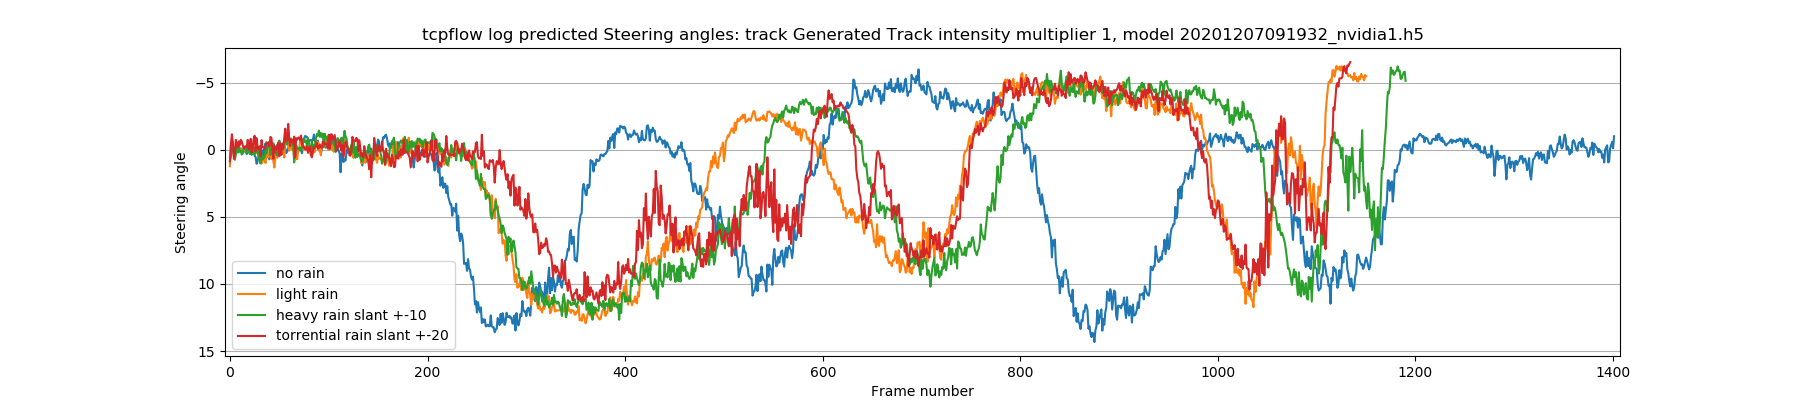
\includegraphics[width=\textwidth]{Figures/sa_GeneratedTrackintensitymultiplier1_20201207091932_nvidia1.h5.png}
 \caption{201207091932\_ nvidia1.h5 steering angle prediction plots for Generated Track, intensity multiplier 1, runs \ref{app_res:81} (no rain), \ref{app_res:72} (light) , \ref{app_res:73} (heavy) and  \ref{app_res:74} (torrential).}
 \label{fig:sa_GeneratedTrackintensitymultiplier1_20201207091932_nvidia1} 
\end{figure}

%%%%%%%%%%%%%%%%%%%%%%%%%%%%%%%%%%%%%%%%%%%%%%%%%%
% BEST nvidia1 MODEL - steering plot
% 201207091932_nvidia1.h5 plots mult 4
% no, light, heavy and torrential rain
%%%%%%%%%%%%%%%%%%%%%%%%%%%%%%%%%%%%%%%%%%%%%%%%%%

\begin{figure}[h!]
 \centering 
 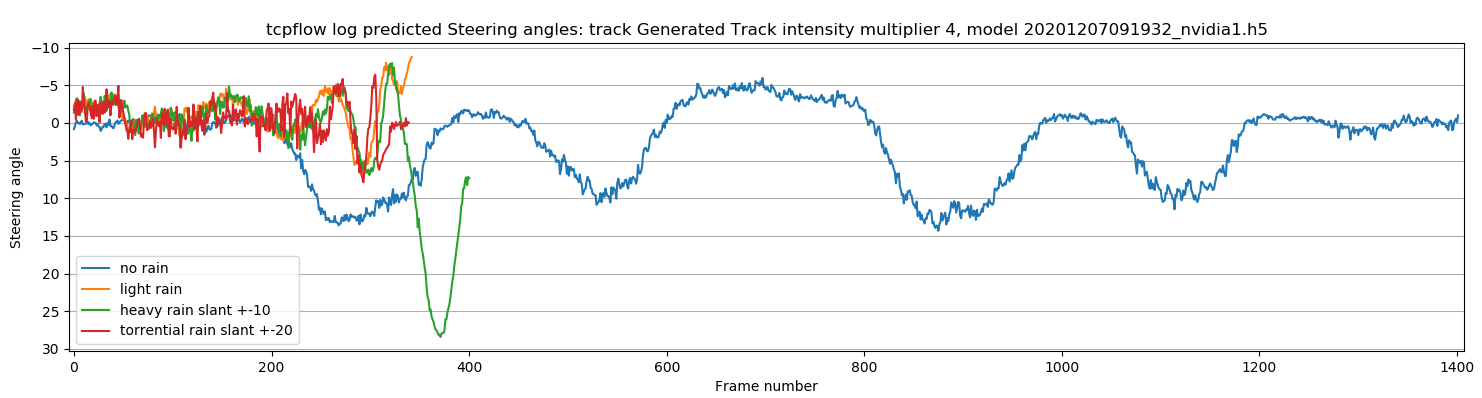
\includegraphics[width=\textwidth]{Figures/sa_GeneratedTrackintensitymultiplier4_20201207091932_nvidia1.h5.png}
 \caption{201207091932\_ nvidia1.h5 steering angle prediction plots for Generated Track, intensity multiplier 4, runs \ref{app_res:81} (no rain),  \ref{app_res:75} (light), \ref{app_res:76} (heavy) and \ref{app_res:77} (torrential). The initial negative (left) steering values predicted by all rain models can be verified in corresponding videos.}
 \label{fig:sa_GeneratedTrackintensitymultiplier4_20201207091932_nvidia1} 
\end{figure}

%%%%%%%%%%%%%%%%%%%%%%%%%%%%%%%%%%%%%%%%%%%%%%%%%%
% BEST nvidia1 MODEL - steering plot
% 201207091932_nvidia1.h5 plots mult 8
% no, light, heavy and torrential rain
%%%%%%%%%%%%%%%%%%%%%%%%%%%%%%%%%%%%%%%%%%%%%%%%%%

\begin{figure}[h!]
 \centering 
 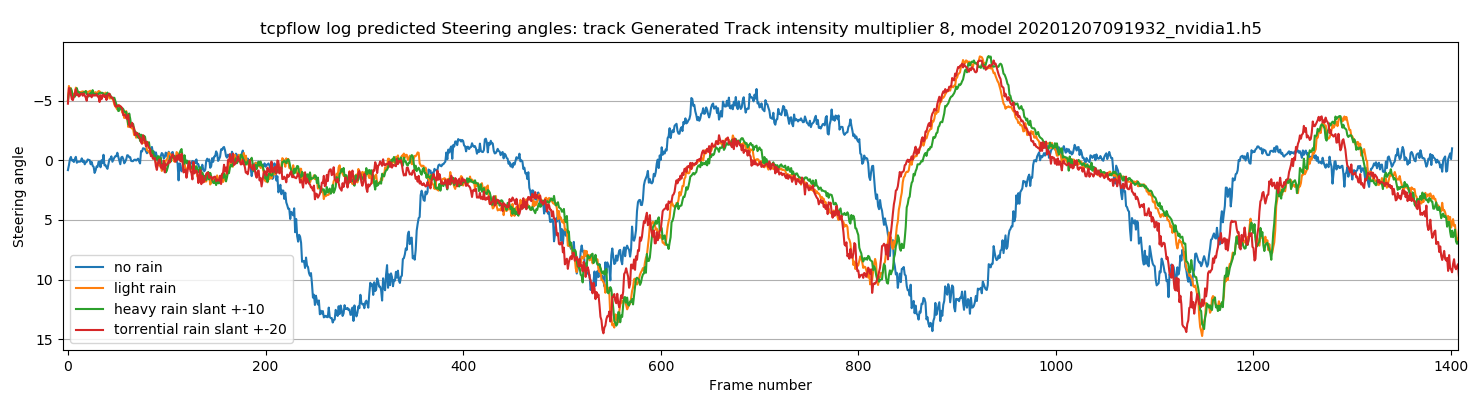
\includegraphics[width=\textwidth]{Figures/sa_GeneratedTrackintensitymultiplier8_20201207091932_nvidia1.h5.png}
 \caption{201207091932\_ nvidia1.h5 steering angle prediction plots for Generated Track, intensity multiplier 8, runs \ref{app_res:81} (no rain),  \ref{app_res:78} (light), \ref{app_res:79} (heavy) and \ref{app_res:80} (torrential).}
 \label{fig:sa_GeneratedTrackintensitymultiplier8_20201207091932_nvidia1} 
\end{figure}

%%%%%%%%%%%%%%%%%%%%%%%%%%%%%%%%%%%%%%%%%
% Phase shift
%%%%%%%%%%%%%%%%%%%%%%%%%%%%%%%%%%%%%%%%%

In figure \ref{fig:sa_GeneratedTrackintensitymultiplier1_20201207091932_nvidia1}, the blue line "no rain" plot shows the circuit curve sequence, with the two right turns (rounded inverted peaks in the positive steering angle range) followed by a left turn (plateau in the negative steering angle range) followed by to right turns. With rain the nvidia1 models understeer (shown by the gentler dip if compared to blue "no rain" light in plot) when taking the first right turn, the "torrential rain" model steering erratically when adjusting the steering before taking the second right turn, while the "light" and "heavy" rain models are smoother. The torrential rain model also takes the second right turn erratically while the other two are smoother. All three models take the long left turn quite well, becoming erratic on the third right turn where all drive off the track. The four plots are overlayed and the circuit geometry and consequent position of model on track can be inferred by the plot shape. The prediction latency (time taken to predict a steering angle given an image) for every weather condition is assumed to be very close in all four runs. This can be verified in data related to Figure \ref{fig:sa_GeneratedTrackintensitymultiplier8_20201207091932_nvidia1} where all models completed the lap and all logs have approximately the same number of frames (x axis maximum value). The horizontal displacement between model prediction plots is due to models going around the track at different speeds. This can be verified in the corresponding videos by pausing all three near frame 1000 (labelled on left image), which shows "light" (\ref{app_res:72} - corresponding to orange line in plot) and "torrential" (\ref{app_res:74} - corresponding to red line in plot) ahead of "heavy" (\ref{app_res:72} - corresponding to green line in plot).

%%%%%%%%%%%%%%%%%%%%%%%%%%%%%%%%%%%%%%%%%
% YOUTUBE STILLS
%%%%%%%%%%%%%%%%%%%%%%%%%%%%%%%%%%%%%%%%%

Figures \ref{fig:youtube20201207091932nvidia1lightrainmult_4_h5}, \ref{fig:youtube20201207091932nvidia1heavy10mult_4_h5} and  \ref{fig:youtube20201207091932nvidia1torrential20mult_4_h5} shows stills from videos generated in runs \ref{app_res:75} (light), \ref{app_res:76} (heavy) and \ref{app_res:77} (torrential) respectively. The runs generated tcpflow (intensity multiplier 4) data used in Figure \ref{fig:sa_GeneratedTrackintensitymultiplier4_20201207091932_nvidia1} orange, green and red lines respectively, all three driving straight off the first right turn, \ref{app_res:77} crashing into a bollard.

%%%%%%%%%%%%%%%%%%%%%%%%%%%%%%%%%%%%%%%%%%%%%%%%
% VIDEO 1 for nvidia1, light rain multiplier 4
%%%%%%%%%%%%%%%%%%%%%%%%%%%%%%%%%%%%%%%%%%%%%%%%

\begin{figure}[h!]
 \centering 
 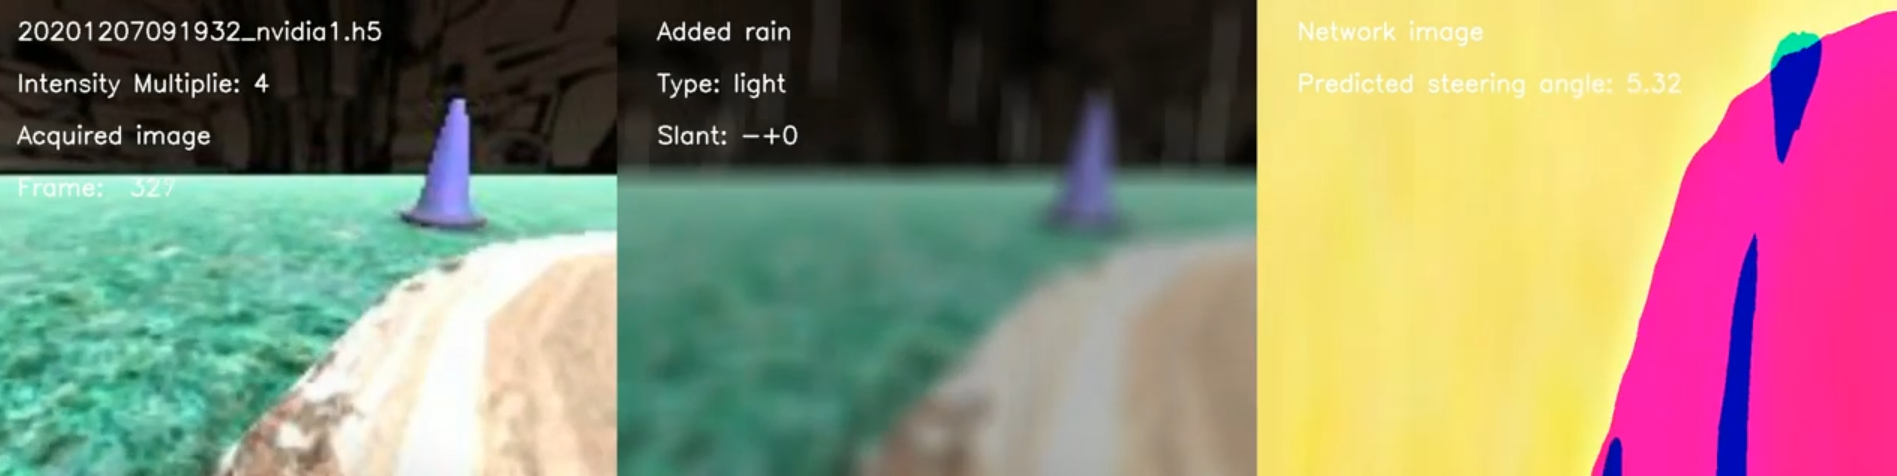
\includegraphics[width=\textwidth]{Figures/youtube20201207091932nvidia1lightrainmult_4_h5.png}
 \caption{Still from video \url{https://youtu.be/qdTA5ho5VOE} showing a self-driving simulated vehicle driving off the Generated Track, where the Unity scene is set to a dark horizon (Setting Skybox Material to SkyCarLightCoversGrey) and the intensity multiplier is set to 4. Rain is set to light. The image sent from Unity simulator over the TCP network is shown on the left, the middle image has added rain and the image on the right is the image presented to the network. The tcpflow log and video were generated in run \ref{app_res:75} and represent the orange line in Figure \ref{fig:sa_GeneratedTrackintensitymultiplier4_20201207091932_nvidia1}.}
 \label{fig:youtube20201207091932nvidia1lightrainmult_4_h5} 
\end{figure}

%%%%%%%%%%%%%%%%%%%%%%%%%%%%%%%%%%%%%%%%%%%%%%%%
% VIDEO 2 for nvidia1, henvy rain multiplier 4
%%%%%%%%%%%%%%%%%%%%%%%%%%%%%%%%%%%%%%%%%%%%%%%%

\begin{figure}[h!]
 \centering 
 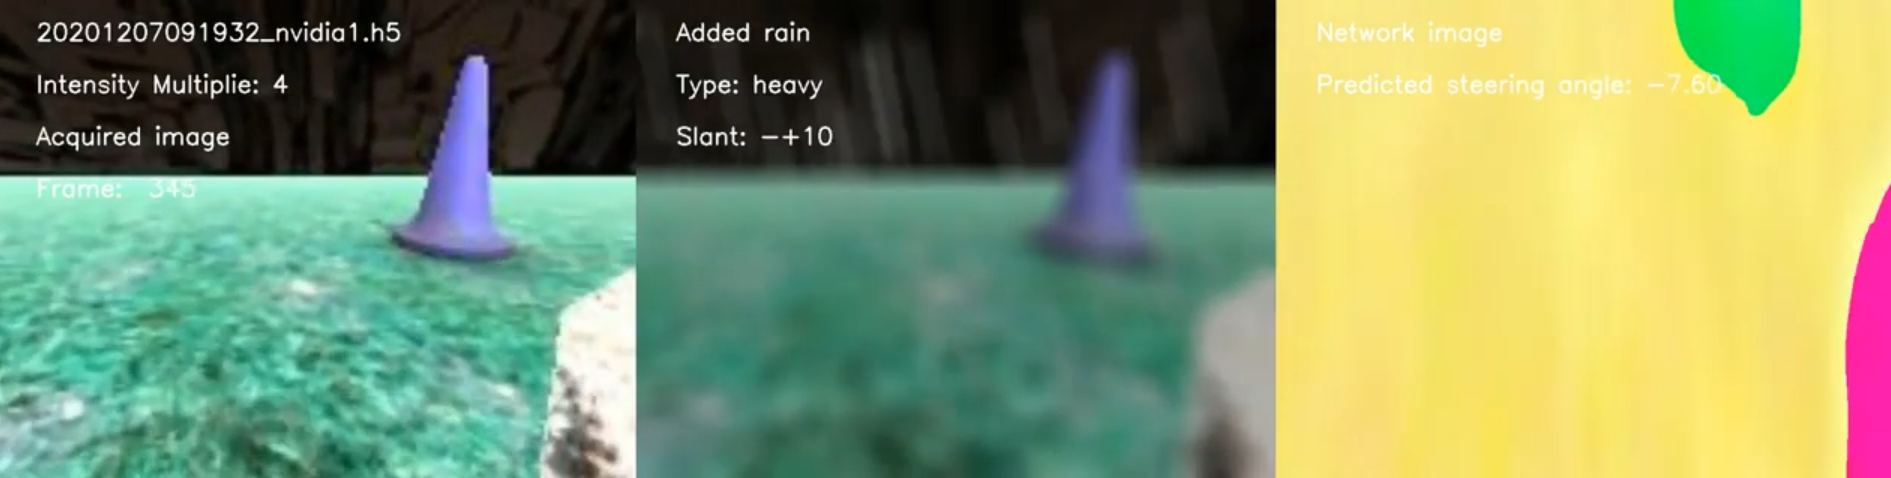
\includegraphics[width=\textwidth]{Figures/youtube20201207091932nvidia1heavy10mult_4_h5.png}
 \caption{Still from \url{https://youtu.be/sKyoke3IO84}. The tcpflow log and video were generated in run \ref{app_res:76} and represent the green line in Figure \ref{fig:sa_GeneratedTrackintensitymultiplier4_20201207091932_nvidia1}}
 \label{fig:youtube20201207091932nvidia1heavy10mult_4_h5} 
\end{figure}

%%%%%%%%%%%%%%%%%%%%%%%%%%%%%%%%%%%%%%%%%%%%%%%%
% VIDEO 3 for nvidia1, torrential rain multiplier 4
%%%%%%%%%%%%%%%%%%%%%%%%%%%%%%%%%%%%%%%%%%%%%%%%

\begin{figure}[h!]
 \centering 
 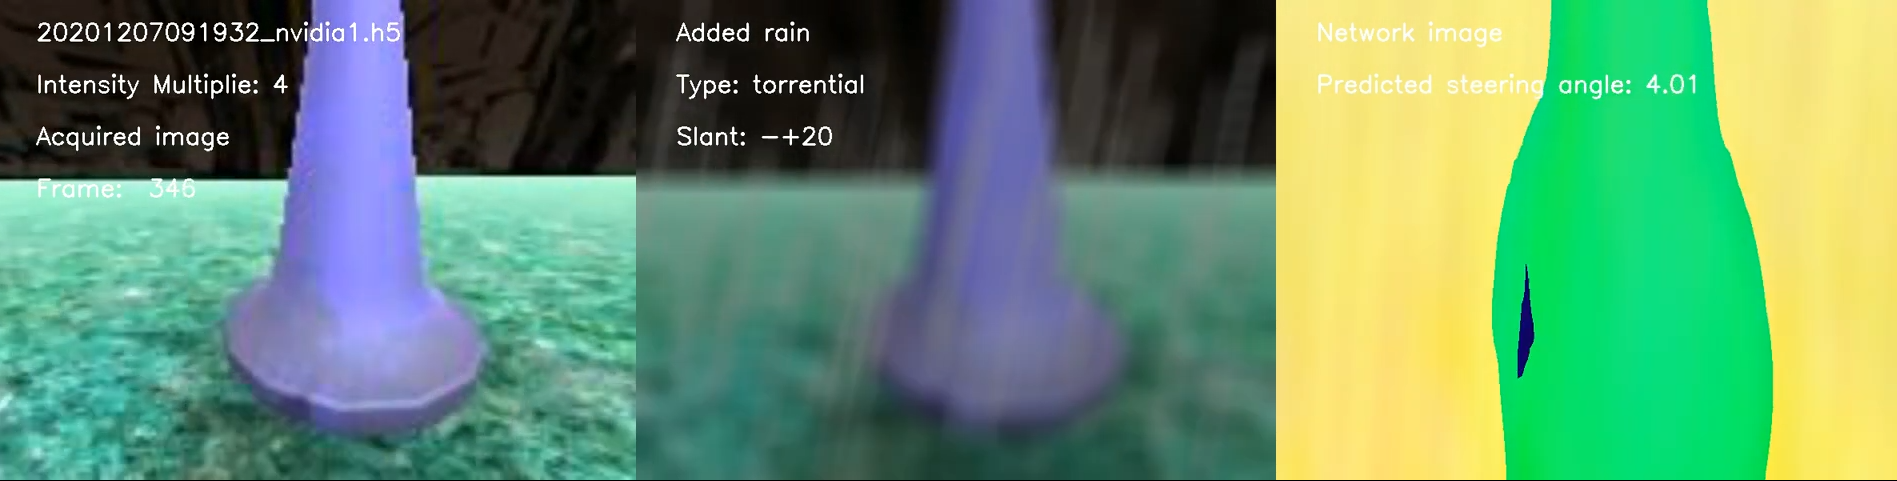
\includegraphics[width=\textwidth]{Figures/youtube20201207091932nvidia1torrential20mult_4_h5.png}
 \caption{Still from \url{https://youtu.be/mDjtnnVZdic}. The tcpflow log and video were generated in run \ref{app_res:77} and represent the red line in Figure \ref{fig:sa_GeneratedTrackintensitymultiplier4_20201207091932_nvidia1}}
 \label{fig:youtube20201207091932nvidia1torrential20mult_4_h5} 
\end{figure}

%%%%%%%%%%%%%%%%%%%%%%%%%%%%%%%%%%%%%%%%%%%
% NVIDIA2 BEST MODEL REALTIME PREDICTIONS
%%%%%%%%%%%%%%%%%%%%%%%%%%%%%%%%%%%%%%%%%%%

%%%%%%%%%%%%%%%%%%%%%%%%%%%%%%%%
% REAL TIME PREDICTIONS NVIDIA2
%%%%%%%%%%%%%%%%%%%%%%%%%%%%%%%%

\subsection{Realtime predictions for best performing nvidia2 model}

Figures
\ref{fig:sa_GeneratedTrackintensitymultiplier1_20201207192948_nvidia2}, 
\ref{fig:sa_GeneratedTrackintensitymultiplier4_20201207192948_nvidia2} and 
\ref{fig:sa_GeneratedTrackintensitymultiplier8_20201207192948_nvidia2} show
plotted steering angles for the best nvidia2 model, on the Generated Track, using different intensity multiplier values (1, 4 and 8) and rain levels (light, heavy, torrential). Blue lines are for "no rain" data generated in run 82 (\ref{app_res:81}) with intensity multiplier 1.  All plots were generated with result\_ plots.py script. The compressed shape of the "no rain" plot in \ref{fig:sa_GeneratedTrackintensitymultiplier8_20201207192948_nvidia2} compared to \ref{fig:sa_GeneratedTrackintensitymultiplier1_20201207192948_nvidia2} and
\ref{fig:sa_GeneratedTrackintensitymultiplier4_20201207192948_nvidia2} is due to the predicted steering angle range for rain models in Figure \ref{fig:sa_GeneratedTrackintensitymultiplier8_20201207192948_nvidia2} being wider, not that predicted angles generated by the models exceed in some cases the maximum Unity simulator steering angle.

%%%%%%%%%%%%%%%%%%%%%%%%%%%%%%%%%%%%%%%%%%%%%%%%%%
% BEST nvidia2 MODEL - steering plot
% 20201207192948_nvidia2 plots mult 1
% no, light, heavy and torrential rain
%%%%%%%%%%%%%%%%%%%%%%%%%%%%%%%%%%%%%%%%%%%%%%%%%%

\begin{figure}[h!]
 \centering 
 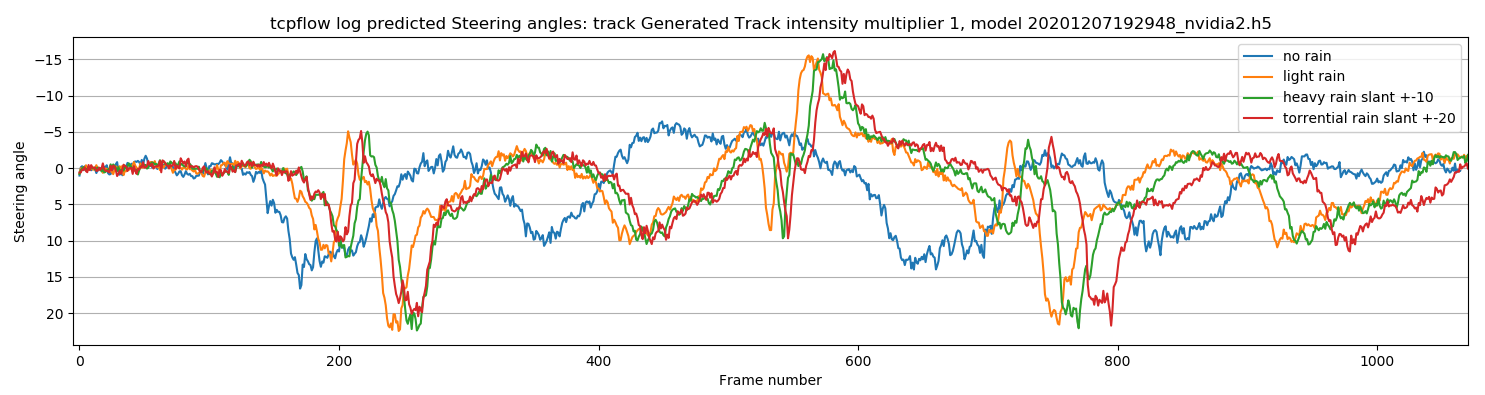
\includegraphics[width=\textwidth]{Figures/sa_GeneratedTrackintensitymultiplier1_20201207192948_nvidia2.h5}
 \caption{nvidia2 20201207192948\_ nvidia2.h5 steering angle prediction plots for Generated Track, intensity multiplier 1, runs \ref{app_res:82} (no rain), \ref{app_res:83} (light) , \ref{app_res:84} (heavy) and  \ref{app_res:85} (torrential). The rain models almost drive off the track near frame 200, then correct themselves. Another near drive-off-the-road incident is recorded near frame 500 followed by another one near frame 700. All rain models recovering and managing to complete the lap.}
 \label{fig:sa_GeneratedTrackintensitymultiplier1_20201207192948_nvidia2} 
\end{figure}

The horizontal shift between light (orange), heavy (green) and torrential rain (red) plots in Figure \ref{fig:sa_GeneratedTrackintensitymultiplier1_20201207192948_nvidia2} is due to the models going around the track at different speeds. In this case it can be verified by pausing videos generated in the corresponding runs \ref{app_res:83}, \ref{app_res:84} and \ref{app_res:85} near frame number 800, labelled on the first image from left to right. At this point, the model subject to light rain is ahead of the model subject to heavy rain, in turn ahead of the model subject to torrential rain, which reflects the displacement of the three plots with orange negative peak to the left ("ahead") of the 800 mark frame, the red negative peak near the 800 axis label and the green negative peak in the middle.

%%%%%%%%%%%%%%%%%%%%%%%%%%%%%%%%%%%%%%%%%%%%%%%%%%
% BEST nvidia2 MODEL - steering plot
% 20201207192948_nvidia2 plots mult 4
% no, light, heavy and torrential rain
%%%%%%%%%%%%%%%%%%%%%%%%%%%%%%%%%%%%%%%%%%%%%%%%%%
% TODO comment on path taken, similar to mult 1
% with less erratic steering
\begin{figure}[h!]
 \centering 
 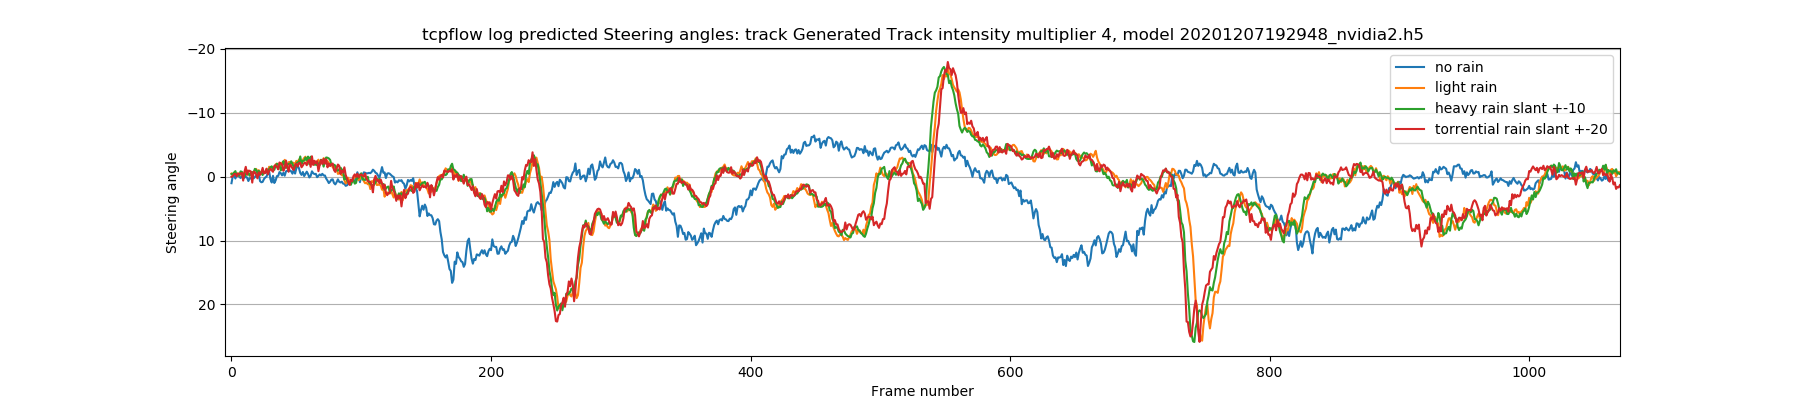
\includegraphics[width=\textwidth]{Figures/sa_GeneratedTrackintensitymultiplier4_20201207192948_nvidia2.h5}
 \caption{nvidia2 20201207192948\_ nvidia2.h5  steering angle prediction plots for Generated Track, intensity multiplier 4, runs \ref{app_res:82} (no rain), \ref{app_res:86} (light) , \ref{app_res:87} (heavy) and  \ref{app_res:88} (torrential).}
 \label{fig:sa_GeneratedTrackintensitymultiplier4_20201207192948_nvidia2} 
\end{figure}

%%%%%%%%%%%%%%%%%%%%%%%%%%%%%%%%%%%%%%%%%%%%%%%%%%
% BEST nvidia2 MODEL - steering plot
% 20201207192948_nvidia2 plots mult 8
% no, light, heavy and torrential rain
%%%%%%%%%%%%%%%%%%%%%%%%%%%%%%%%%%%%%%%%%%%%%%%%%%

\begin{figure}[h!]
 \centering 
 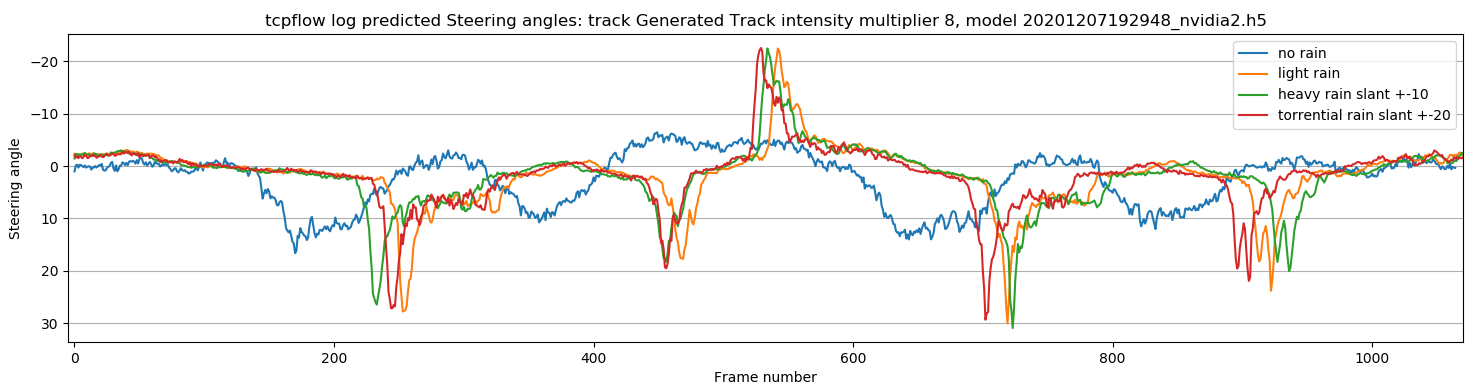
\includegraphics[width=\textwidth]{Figures/sa_GeneratedTrackintensitymultiplier8_20201207192948_nvidia2.h5}
 \caption{nvidia2 20201207192948\_ nvidia2.h5 steering angle prediction plots for Generated Track, intensity multiplier 8, runs \ref{app_res:82} (no rain), \ref{app_res:89} (light) , \ref{app_res:90} (heavy) and  \ref{app_res:91} (torrential).}
 \label{fig:sa_GeneratedTrackintensitymultiplier8_20201207192948_nvidia2} 
\end{figure}

The general shape of the negative and positive peaks for the best nvidia2 models driving in the rain reflect the more abrupt steering angles predicted by the model in situations when they were about to drive off the road. The nvidia1 model, when it did manage to complete a lap in the rain (Figure \ref{fig:sa_GeneratedTrackintensitymultiplier8_20201207091932_nvidia1}) presented comparatively smoother steering.

%%%%%%%%%%%%%%%%%%%%%%%%%%%%%%%%%%%%%%%%%%%%%%%%%%%%%%%%%%%%%%%%%%%
% YOUTUBE STILLS Best performing nvidia2 20201207192948_nvidia2
%%%%%%%%%%%%%%%%%%%%%%%%%%%%%%%%%%%%%%%%%%%%%%%%%%%%%%%%%%%%%%%%%%%

% Redundant, the following figure
%\begin{figure}[ht]
% \centering 
% \includegraphics[width=\textwidth]{Figures/youtube20%201207192948_nvidia2torrential20mult_8_h5.png}
% \caption{Youtube video still showing the %20201207192948\_ nvidia2.h5 model predictions around %Generated Track in torrential +-2- degree slant rain %(\url{https://youtu.be/W1eRN5DWPXw})}
% \label{fig:youtube20201207192948_nvidia2torrential20%mult_8_h5} 
%\end{figure}

Figure \ref{fig:20201207192948_nvidia2_mult_1_4_8_light} in appendix \ref{AppendixD} shows three rows of stills, generated in runs 83 (\ref{app_res:83}), 86 (\ref{app_res:86}) and 89 (\ref{app_res:89}  for light rain and intensity multipliers 1, 4 and 8 respectively, The data generated was used to plot the orange lines in figures  \ref{fig:sa_GeneratedTrackintensitymultiplier1_20201207192948_nvidia2}, 
\ref{fig:sa_GeneratedTrackintensitymultiplier4_20201207192948_nvidia2} and 
\ref{fig:sa_GeneratedTrackintensitymultiplier8_20201207192948_nvidia2} for the best performing nvidia2 model. The sequence highlights the effect of preprocessing, when noise has been applied in equal measure to images generated with different intensity multipliers, where in the first row (intensity multiplier 1), the road markings are still visible, in the second row (intensity multiplier 4) the road markings are hardly visible and the reflection in the middle of the lane is generating a continuous vertical stripe on the network image, and in the third row, where the reflection on the road is such, road markings are no longer visible.

This concluded the 32 recorded realtime runs in the rain for the best performing models. One more video was generated with Kazam, showing 4 concurrent predictions on the same Generated Track using built in SDSandbox functionality. Figure  \ref{fig:2948x3_1932x1_genTrack}  shows a still from video \url{https://youtu.be/ayESXH9zZdM}.
Bottom left is best nvidia2 20201207192948\_ nvidia2.h5 model running predictions for no rain, bottom right is 20201207192948\_ nvidia2.h5 light rain zero slant. Top left is best nvidia1   
20201207091932\_ nvidia1.h5 model, light rain zero slant (crashes on third right turn), top right is 20201207192948\_ nvidia2.h5 torrential rain -+20 degree slant. This provides a qualitative analysis of how well the models are steering, where the bottom left nvidia1 in no rain is noticeably the smoothest steering model.

%%%%%%%%%%%%%%%%%%%%%%%%%%%%%%%%%%
%% SYNTHETIC DATASET PREDICTIONS
%%%%%%%%%%%%%%%%%%%%%%%%%%%%%%%%%%

\subsection{Synthetic dataset predictions}

%%%%%%%%%%%%%%%%%%
% RESULTS TABLE
%%%%%%%%%%%%%%%%%%

% Table generated with steerlib.py
\begin{table}[]
\begin{center}
\begin{tabular}{|l|l|l|l|l|l|}
\hline
\multicolumn{6}{|c|}{Goodness-of-steer results - Generated Track and Generated Road SDSandbox logs} \\ \hline

% 1 Log: Unity log location (image plus .json files)
% 1 Filename:   Download  D1  Udacity real world dataset
% 2 Model:    D2  Udacity simulator data
% 3 Rain Type: D3  Udacity real and simulator data
% 4 Slant: Turk dry/rainy Ford dataset
% 5.GOS: Goodness of steer

% Generated Track log number of image files
% $ ls -l ../../dataset/unity/genTrack/genTrackOneLap/logs_Wed_Nov_25_23_39_22_2020/*.jpg | wc -l
% 1394
% Generated Road log number of image files
% $ ls -l ../../dataset/unity/genRoad/logs_Fri_Jul_10_09_16_18_2020/*.jpg | wc -l
% 19679

\multicolumn{6}{|c|}{Generated Track log: logs\_ Wed\_ Nov\_ 25\_ 23\_ 39\_ 22\_ 2020 (1394 images)} \\ \hline
ID & Keras model file name & Model & Rain Type & Slant & $g_s$ \\ \hline
% GENERATED TRACK
1 & 20201207192948\_ nvidia2.h5 & nvidia2 :) &  & 0 & 1.68 * \\ \hline
2 & 20201207192948\_ nvidia2.h5 & nvidia2 & light & 0 & 2.12 \\ \hline
3 & 20201207192948\_ nvidia2.h5 & nvidia2 & heavy & 10 & 2.17 \\ \hline
4 & 20201207192948\_ nvidia2.h5 & nvidia2 & torrential & 20 & 2.30 \\ \hline
5 & 20201207091932\_ nvidia1.h5 & nvidia1 &  & 0 & 1.82 * \\ \hline
6 & 20201207091932\_ nvidia1.h5 & nvidia1 & light & 0 & 2.11 \\ \hline
7 & 20201207091932\_ nvidia1.h5 & nvidia1 & heavy & 10 & 2.13 \\ \hline
8 & 20201207091932\_ nvidia1.h5 & nvidia1 & torrential & 20 & 2.28 \\ \hline
9 & 20201207201157\_ nvidia\_ baseline.h5 & nvidia2\_ baseline &  & 0 & 2.32 * \\ \hline
10 & 20201207201157\_ nvidia\_ baseline.h5 & nvidia2\_ baseline & light & 0 & 3.12 \\ \hline
11 & 20201207201157\_ nvidia\_ baseline.h5 & nvidia2\_ baseline & heavy & 10 & 3.17 \\ \hline
12 & 20201207201157\_ nvidia\_ baseline.h5 & nvidia2\_ baseline & torrential & 20 & 3.39 \\ \hline
13 & 20201120171015\_ sanity.h5 & nvidia1 :( &  & 0 & 5.03 * \\ \hline
14 & 20201120171015\_ sanity.h5 & nvidia1 & light & 0 & 3.11 \\ \hline
15 & 20201120171015\_ sanity.h5 & nvidia1 & heavy & 10 & 3.07 \\ \hline
16 & 20201120171015\_ sanity.h5 & nvidia1 & torrential & 20 & 3.00 \\ \hline
% GENERATED ROAD
\multicolumn{6}{|c|}{Generated Road log:  logs\_ Fri\_ Jul\_ 10\_ 09\_ 16\_ 18\_ 2020 (19679 images)} \\ \hline
ID & Keras model file name & Model & Rain Type & Slant & $g_s$ \\ \hline
% NVIDIA2
17 & 20201207192948\_ nvidia2.h5 & nvidia2 :) &  & 0 & 2.99 * \\ \hline  % drove 16 minutes on this road 1 & https://youtu.be/z9nILq9dQfI
18 & 20201207192948\_ nvidia2.h5 & nvidia2 & light & 0 & 3.20 \\ \hline
19 & 20201207192948\_ nvidia2.h5 & nvidia2 & heavy & 10 & 3.22 \\ \hline
20 & 20201207192948\_ nvidia2.h5 & nvidia2 & torrential & 20 & 3.27 \\ \hline
% NVIDIA1
21 & 20201207091932\_ nvidia1.h5 & nvidia1 &  & 0 & 3.87 * \\ \hline
22 & 20201207091932\_ nvidia1.h5 & nvidia1 & light & 0 & 3.75 \\ \hline
23 & 20201207091932\_ nvidia1.h5 & nvidia1 & heavy & 10 & 3.70 \\ \hline
24 & 20201207091932\_ nvidia1.h5 & nvidia1 & torrential & 20 & 3.57 \\ \hline
% NVIDIA_BASELINE
25 & 20201207201157\_ nvidia\_ baseline.h5 & nvidia2\_ baseline :( &  & 0 & 5.51 * \\ \hline
26 & 20201207201157\_ nvidia\_ baseline.h5 & nvidia2\_ baseline & light & 0 & 4.97 \\ \hline
27 & 20201207201157\_ nvidia\_ baseline.h5 & nvidia2\_ baseline & heavy & 10 & 4.98 \\ \hline
28 & 20201207201157\_ nvidia\_ baseline.h5 & nvidia2\_ baseline & torrential & 20 & 5.05 \\ \hline
% SANITY (NVIDIA1)
29 & 20201120171015\_ sanity.h5 & nvidia1 &  & 0 & 3.85 * \\ \hline
30 & 20201120171015\_ sanity.h5 & nvidia1 & light & 0 & 3.06 \\ \hline
31 & 20201120171015\_ sanity.h5 & nvidia1 & heavy & 10 & 3.05 \\ \hline
32 & 20201120171015\_ sanity.h5 & nvidia1 & torrential & 20 & 3.02 \\ \hline
%   compare to genTrackOneLap_logs_Wed_Nov_25_23_39_22_2020_ground_truth_steering_angles.png
\end{tabular}
\end{center}
\caption{Goodness-of-Steer $g_s$ results for best performing nvidia2 and nvidia1, plus "sanity" and nvidia\_ baseline for comparison, obtained from one lap of Generated Track (logs\_ Wed\_ Nov\_ 25\_ 23\_ 39\_ 22\_ 2020, rows 1 to 16) and one stretch of Generated Road (logs\_ Fri\_ Jul\_ 10\_ 09\_ 16\_ 18\_ 2020, rows 17 to 32). Asterisks in $g_s$ column indicate dry weather. Smiley face :) in Model column indicate best (lowest) $g_s$ score. Sad face :( in Model column indicates worst (highest) $g_s$ scores. The logs containing labelled image data used to compute the $g_s$ scores were generated with Unity intensity multiplier 1 and Skybox-Material set to Default-Skybox, the default sunny dry weather.}
\label{table:goodness-of-steer}
\end{table}

Table \ref{table:goodness-of-steer} shows Goodness-of-Steer results obtained for 32 sets of predictions, for four networks and two SDSandbox track logs, that is, the results were generated by running predictions on synthetic datasets, which contain ground truth steering values, like plotted in Figure \ref{fig:genTrackOneLap_logs_Wed_Nov_25_23_39_22_2020_ground_truth_steering_angles}. It is important to stress these are not realtime predictions, and the Unity simulator was not running in this case.

The networks are the best performing nvidia2 (obtained in run 62 - \ref{app_res:62}), the second best performing nvidia1 (obtained in run 49 - \ref{app_res:49}), "sanity check" (obtained in run 36 - \ref{app_res:36}) and nvidia\_ baseline (obtained in run 68 - \ref{app_res:68}). Table data and steering angle plots was generated with steerlib.py script written for this project. The track logs are for Generated Track (one lap) and Generated Road (one stretch). There are 32 rows, each sequence of four (1-4, 5-8 and so on) representing one model subject to sunny weather followed by 3 types of rain predicting steering angles for one log. 

nvidia2 predicted steering angle values used to generate $g_s$ scores in rows 1, 2, 3 and 4, for the Generated Track log are plotted in Figure  \ref{fig:sa_Generated_Track_20201207192948_nvidia2.h5}. The "no rain" predictions in row 1 (orange line on the plot), which has the lowest overall (1.68) $g_s$ score, is clearly the closest to the ground truth blue line, while the predictions for images containing light, heavy and torrential rain are tightly overlapped (green, red an violet lines, $g_s$ scores 2.12, 2.17, 2.30 respectively) are understeering on all turns (slightly above right turn ground truth plot in right turn sections and below ground truth plot in the left turn section. The understeering aspect was also noted in realtime predictions with respect to rainy predictions compared to best-run dry weather predictions as shown in Figures \ref{fig:sa_GeneratedTrackintensitymultiplier1_20201207192948_nvidia2}, 
\ref{fig:sa_GeneratedTrackintensitymultiplier4_20201207192948_nvidia2} and 
\ref{fig:sa_GeneratedTrackintensitymultiplier8_20201207192948_nvidia2}.


% NB All 6 Generated Track rain/multiplier plots generated with code from commit 610939215 (result_plots.py) 

% Image template
%\begin{figure}[ht]
% \centering 
% \includegraphics[width=\textwidth]{Figures/a}
% \caption{Description}
% \label{fig:} 
%\end{figure}

% Plots generated with steerlib.py, commit 8693713


%%%%%%%%%%%%%%%%%%%%%%%%%%%%%%%%%%%%%%
% NVIDIA2 PLOTS
%%%%%%%%%%%%%%%%%%%%%%%%%%%%%%%%%%%%%%
\begin{figure}[h!]
 \centering 
 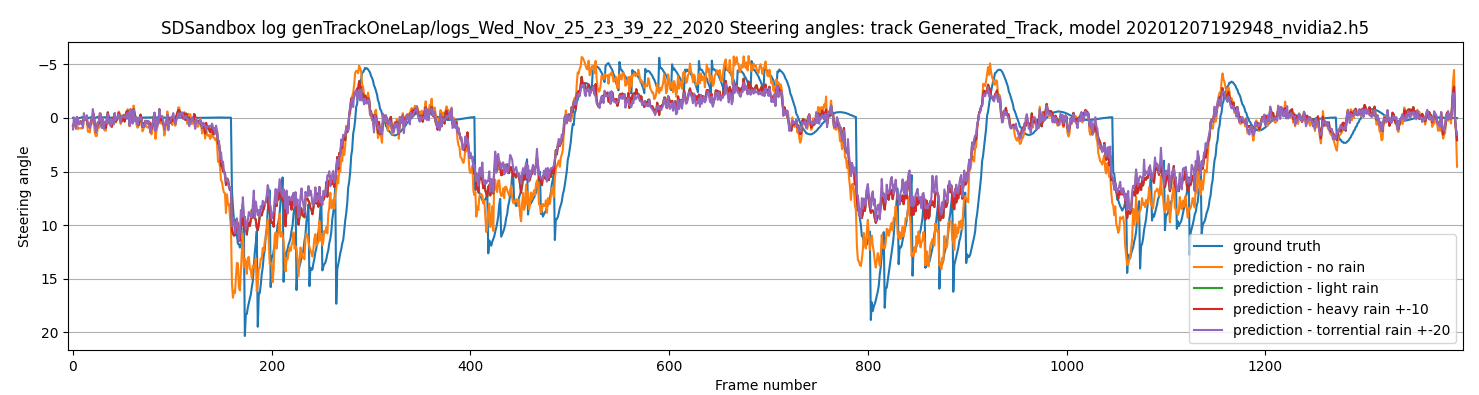
\includegraphics[width=\textwidth]{Figures/sa_Generated_Track_20201207192948_nvidia2.h5.png}
 \caption{Plots of SDSandbox log logs\_ Wed\_ Nov\_ 25\_ 23\_ 39\_ 22\_ 2020 ground truth plus steering angle predictions used to generate $g_s$ values for model nvidia2 in rows 1, 2, 3 and 4 in table \ref{table:goodness-of-steer}}
 \label{fig:sa_Generated_Track_20201207192948_nvidia2.h5} 
\end{figure}

For the best nvidia1 model, predicted steering angle values used to generated $g_s$ values in rows 5, 6 and 7 and 8 are plotted in Figure \ref{fig:sa_Generated_Track_20201207091932_nvidia1.h5}. The "no rain" orange plot corresponding to row 5 shows some understeering, with the orange plot not following the ground truth blue plot as closely as the corresponding nvidia2 plot in Figure \ref{fig:sa_Generated_Track_20201207192948_nvidia2.h5} . This is reflected in the slighty higher 1.82 $g_s$ score in comparison to corresponding nvidia2 result in row 1. Predictions for rain follow the close overlap observed for the nvidia2 models, the $g_s$ scores for nvidia1 rain predictions are better than the corresponding nvidia2 values. The distinguishing feature being the closer predictions to the ground truth for the left turn section. This is consistent with the nvidia1 realtime plots in Figure  \ref{fig:sa_GeneratedTrackintensitymultiplier8_20201207091932_nvidia1}, where the nvidia1 model steering angle plot in the closest to the profile of the left turn taken by the model predicing steering in dry weather (blue line), compared to all other equivalent realtime plots.

%%%%%%%%%%%%%%%%%%%%%%%%%%%%%%%%%%%%%%
% NVIDIA1 PLOTS
%%%%%%%%%%%%%%%%%%%%%%%%%%%%%%%%%%%%%%
\begin{figure}[h!]
 \centering 
 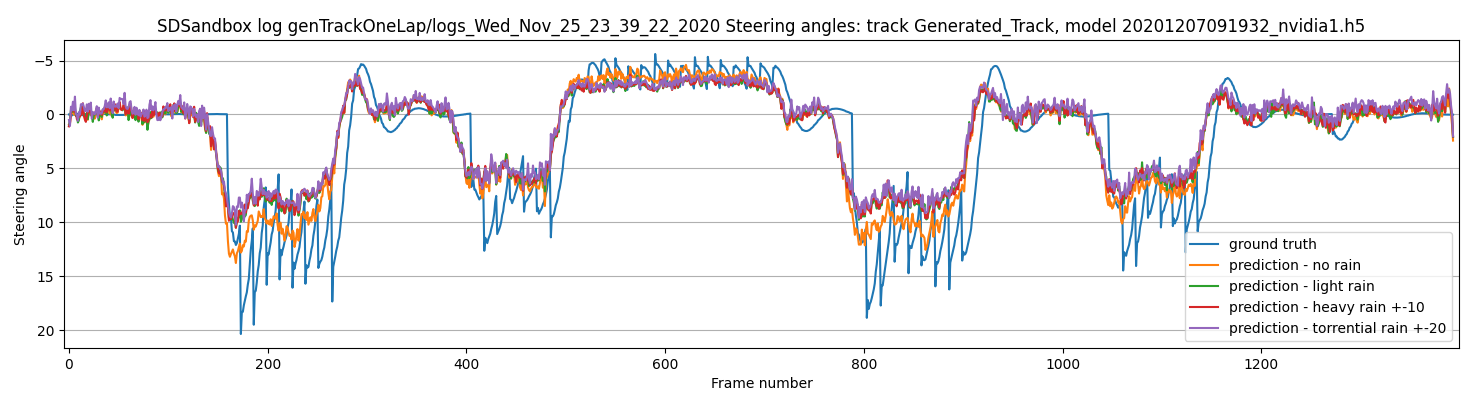
\includegraphics[width=\textwidth]{Figures/sa_Generated_Track_20201207091932_nvidia1.h5.png}
 \caption{Plots of SDSandbox log logs\_ Wed\_ Nov\_ 25\_ 23\_ 39\_ 22\_ 2020 ground truth plus steering angle predictions used to generate $g_s$ values for model nvidia1 in rows 5, 6, 7 and 8 in table \ref{table:goodness-of-steer}}
 \label{fig:sa_Generated_Track_20201207091932_nvidia1.h5} 
\end{figure}

%%%%%%%%%%%%%%%%%%%%%%%%%%%%%%%%%%%%%%
% NVIDIA_BASELINE PLOTS
%%%%%%%%%%%%%%%%%%%%%%%%%%%%%%%%%%%%%%
Rows 9, 10, 11 and 12 represent data generated from the \textit{nvidia2\_ baseline} model, this is the 20201207201157\_ nvidia\_ baseline.h5 trained on run 68 (\ref{app_res:68}), commit b1af57c, and is the same architecture as nvidia1, the only difference being it was trained with a 0.00001 learning rate, while the other 3 models tested were trained with 0.0001 learning rate. This nvidia\_ baseline model was erroneously trained with nvidia1 geometry. This means that at inference time, the nvidia1 geometry must be used. When the steerlib.py script (commit 8693713) was run to generate the plots, the incorrect parameter \textit{nvidia2\_ baseline} typo was passed to the Augmentation library, the model geometry was not found and nvidia1 geometry was used by default. So the nvidia2\_ baseline model should be interpreted in this context as nvidia1 trained with 0.00001 learning rate over 5 epochs. The plots show in addition to previous observations on close overlaps of steering angle predictions for rain, and no rain plot following ground truth more closely than rainy predictions, the general trend in this plot is severe understeering on left and right curves, the steering angle predictions rarely being negative values, this is reflected on the worst $g_s$ scores for steering angle predictions in the rain for Generated Track log and could be attributed to the learning rate used when training the model.

\begin{figure}[h!]
 \centering 
 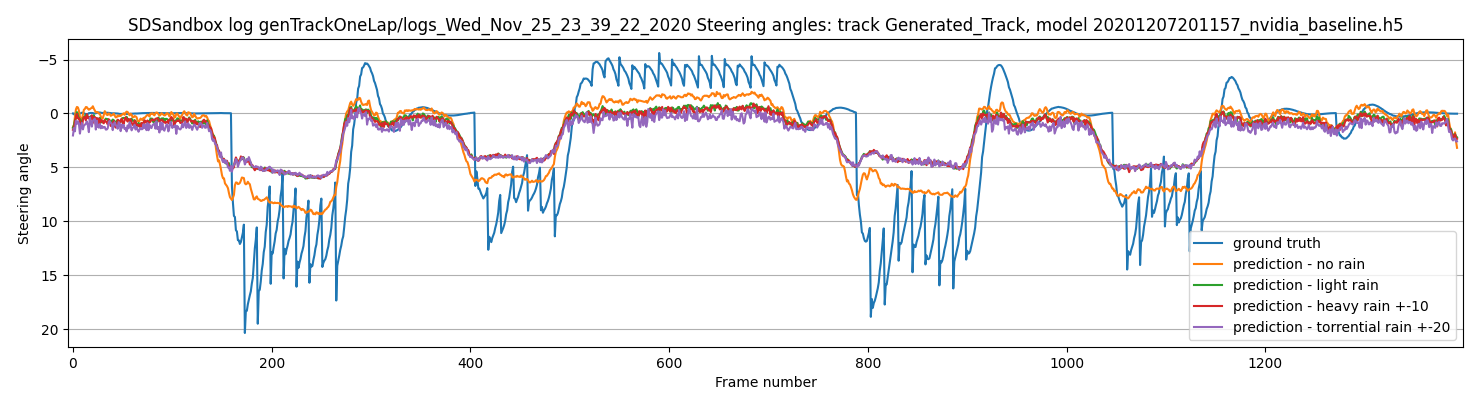
\includegraphics[width=\textwidth]{Figures/sa_Generated_Track_20201207201157_nvidia_baseline.h5.png}
 \caption{Plots of SDSandbox log logs\_ Wed\_ Nov\_ 25\_ 23\_ 39\_ 22\_ 2020 ground truth plus steering data predictions used to generate gos values for model nvidia\_ baseline in rows 9, 10, 11  and 12 in table \ref{table:goodness-of-steer}}
 \label{fig:sa_Generated_Track_20201207201157_nvidia_baseline.h5} 
\end{figure}


%%%%%%%%%%%%%%%%%%%%%%%%%%%%%%%%%%%%%%
% SANITY PLOTS
%%%%%%%%%%%%%%%%%%%%%%%%%%%%%%%%%%%%%%
sanity predicted steering angles for Generated Track log used to generate $g_s$ scores in rows 13, 14, 15 and 16 are plotted in figure \ref{fig:sa_Generated_Track_20201120171015_sanity.h5} 
This model, unlike the previous 3 trained on genTrack data, was trained on the log\_ sample dataset (small\_ looping\_ course, run \ref{app_res:36}), which is the same as the Generated Track course with the addition of trees, bushes, mounts and foliage. The "no rain" plot shows the model oversteering on right turns and understeering on the left turn, reflected in the worst overall $g_s$ score (5.03) for Generated Track log "no rain" predictions, though the closely overlapped rainy predictions achieve better scores (3.11, 3.07 and 3.00) than nvidia2\_ baseline (3.12, 3.17 and 3.39) suggesting the lower learning rate value used for the nvidia2\_ baseline model may be the cause.

\begin{figure}[h!]
 \centering 
 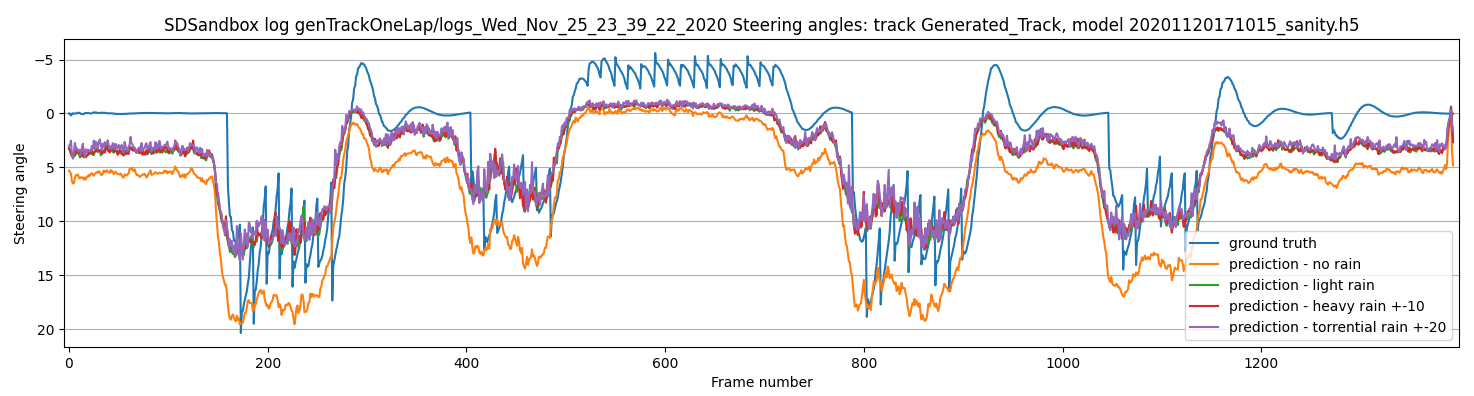
\includegraphics[width=\textwidth]{Figures/sa_Generated_Track_20201120171015_sanity.h5.png}
 \caption{Plots of SDSandbox log logs\_ Wed\_ Nov\_ 25\_ 23\_ 39\_ 22\_ 2020 ground truth plus steering data predictions used to generate gos values for model sanity in rows 13, 14,15  and 16 in table \ref{table:goodness-of-steer}}
 \label{fig:sa_Generated_Track_20201120171015_sanity.h5} 
\end{figure}

No plots were generated for rows 17 to 32 because given the number of images (19679), the plotted lines would have been much thicker and not made good material for qualitative analysis (see Figure  \ref{fig:20201207192948_nvidia2_dry_genRoad_full}). Given there are several right and left turns, in the Generated Road log used for predictions to obtain this set of $g_s$ scores, the higher score (worse) values seem justified as there are more steering adjustments to be made along the path compared to the Generated Track circuit. The overall trend being, nvidia2 had the best overall (2.99) score, nvidia2\_ baseline had the worst overall (5.51) score, the sanity model had the best overall rainy prediction scores (3.06, 3.05 and 3.02) and nvidia2\_ baseline had the corresponding worst overall (4.97, 4.98 and 5.05), making nvidia2\_ baseline the overall worst performing network for the Generated Road log, noting the learning rate used for this model was different. 


%%%%%%%%%%%%%%%%%%%%%%%%%%%%%%%%%%%%%%%%%%%%%%%%%%%
% Modifications to original source codes
%%%%%%%%%%%%%%%%%%%%%%%%%%%%%%%%%%%%%%%%%%%%%%%%%%%

\section{Modifications to original source codes}
Modifications were required to original source codes that were integrated in this project: \cite{Saxena2017} (Automold), \cite{Naoki2016} (Augmentation), and \cite{SDSandboxSim} (SDSandbox). The automold library is designed to process lists of RGB images represented as numpy (\cite{harris2020array}) arrays. Function \textit{add\_ rain\_ single} was added to Automold.py script to deal with image arrays being processed one at a time when running predictions with added rain in real time. The Augmentation library was incorporated into a python class in Augmentation.py. The original code was modified such that before beginning augmentation, the image is resized to the expected acquired size as produced by camera (e.g. 320x160 for nvidia2 and nvidia\_ baseline models, 160x120 for nvidia1 and sanity models). This was set as a configuration parameter in the SDSandbox script conf.py. The preprocessing was modified to use top and bottom crop sizes from configurable values set in conf.py.  
 
The modifications to SDSandbox were made to scripts conf.py, predict\_ client.py and train.py. conf.py was modified such that parameters could be set then shared across function calls. For instance, when running script predict\_ client.py in \ref{app_res:83}, conf.py is used to store rain, slant and record arguments in configuration settings, further checked throughout the running script to determine actions. Image geometry parameters image width, height, depth, expected network width and height, top and bottom crop values for preprocessing was stored as python lists in conf.py. This ensured that the same image geometry was being used during training and inference time for the specified network. This is set with command line argument --modelname for inference in predict\_ client.py (e.g. \ref{app_res:83}) and --model in train.py (e.g. \ref{app_res:92}) for training.  
predict\_ client.py was modified to use the Augmentation class, the modified conf.py and the Automold library, to preprocess image with correct geometry, before presenting to network for prediction, and to add rain to images. The script was also modified to generate videos making use of the RecordVideo.py class.  
train.py was modified to take additional command line arguments --aug and --preproc to determine if augmentation and preprocessing were to be performed for testing. The script was also modified to save: the training history, a history training image and a training log file. Network image geometries settings in conf.py are also used by train.py in the modified version.
